\documentclass[12pt,letterpaper]{article}

% Packages
\usepackage[utf8]{inputenc}
\usepackage[T1]{fontenc}
\usepackage{geometry} 
\usepackage{pdfpages}
\usepackage{framed}
\usepackage{placeins}
\usepackage[textsize=tiny,textwidth=2cm]{todonotes}
\usepackage[colorlinks=true,linkcolor=blue,urlcolor=blue,citecolor=blue,anchorcolor=blue]{hyperref}
\usepackage[figure,table]{hypcap}

\usepackage{tikz}
\usetikzlibrary{fit}
\usetikzlibrary{calc}
\usetikzlibrary{shapes.geometric, arrows}
\definecolor{colorStartStop}{RGB}{118, 140, 186}
\definecolor{colorDecision}{RGB}{164, 185, 166}
\definecolor{colorInfluence}{RGB}{169, 203, 169}
\definecolor{colorProcess}{RGB}{205, 183, 196}
\tikzstyle{startstop} = [rectangle, rounded corners, minimum width=3cm, minimum height=1cm,text centered, draw=colorStartStop, fill=colorStartStop]
\tikzstyle{process} = [rectangle, rounded corners, minimum width=3cm, minimum height=1cm,text centered, draw=colorProcess, fill=colorProcess]
\tikzstyle{influence} = [rectangle, rounded corners, minimum width=3cm, minimum height=1cm,text centered, draw=colorInfluence, fill=colorInfluence]
\tikzstyle{decision} = [diamond, minimum width=3cm, minimum height=1cm, text centered, draw=colorDecision, fill=colorDecision]

\usepackage[backend=biber]{biblatex}
\addbibresource{references.bib}
\AtEveryBibitem{
  \clearfield{pages}
  \clearfield{number}
  \clearfield{issn}
  \clearfield{month}
  \clearfield{day}
  \clearfield{volume}
  \clearfield{pmid}
}
\setcounter{biburlnumpenalty}{9000}
\setcounter{biburlucpenalty}{9000}
\setcounter{biburllcpenalty}{9000}

% Page Layout
\geometry{top=1in, bottom=1in, left=1in, right=1in}

\begin{document}

\title{Medicine Thoughts: A Mixed Methods Review and Proposed Framework for MDMA-Therapy and MDMA-Assisted Methods of Self-knowledge, Meaning, and Connection}
\author{
    Mark Groeneveld\thanks{Email: \href{mailto:mgroeneveld@protonmail.ch}{mgroeneveld@protonmail.ch}}
    \and Thomas Harper, M.S.W.\thanks{Master of Social Work; Email: \href{mailto:thomasharpertherapist@gmail.com}{thomasharpertherapist@gmail.com}}
}
\date{DRAFT Version 0.2 \today}
\maketitle{
    \begin{center}
        All rights reserved in draft form. Do not distribute without permission in draft form.

        \vspace{\baselineskip}

        We welcome comments at \href{mailto:mgroeneveld@protonmail.ch}{mgroeneveld@protonmail.ch}.

        % This work is licensed under \href{https://creativecommons.org/licenses/by/4.0/}{CC BY 4.0}.
        
        \vspace{\baselineskip}

        Please share this document via this link to ensure people have the latest version: \todo{Host this document on PsyArXiv.} This site also keeps track of download counts, which informs us how many people are using the guide and how worthwhile it is to keep it updated with new research.

        \vspace{\baselineskip}

        If you find this manual of value, we would deeply appreciate it if you sent a tip to mgroeneveld@protonmail.ch on Zelle, Venmo, or Paypal. We spent about 400 hours writing this, not including much of the acquisition of relevant skills and knowledge.
    \end{center}
}

\begin{abstract}
    
\end{abstract}
\newpage

\tableofcontents
\newpage

\section*{META (Remove before publication)}
Goals:
\begin{itemize}
    \item Broad audience -> Avoid language or references that may unnecessarily activate challenging schemas for various large groups. Avoid unnecessarily technical language. Minimize length so people aren't scared away and can readily digest it. Conciseness and lack of useless wordiness for better readability. Audience feels guide is reputable, safe, and high quality.
    \item Achievable writing task (knowledge and time) -> Only attempt to write manual for an audience open to a neurological/egalitarian framing of trauma and healing. I can only write recommendations that I know are good within the culture I live in. It might also be appealing to the more diverse, spreading Modern Global Individualist culture? Probably less applicable to more different cultures.
    \item Maximize healing and minimize risk -> Comprehensive. Rigorous. Proper balance between risk-warning language and healing-hopeful language so we don't unnecessarily scare people away OR fail to adequately warn about real risks. Most people doing healing need a lot more than reconsolidation; include broadly useful resources on emotional skills.
    \item Avoid legal risk -> Disclaimer and wording.
    \item Improve authors' understanding of concepts -> Rigor. Comprehensiveness. Usefulness to broad audience.
    \item Improve authors' reputation -> Publish in a journal (J. Psychedelic Psychiatry looks like a good fit. If all else fails, can still put it on Psyarxiv.). Rigor. Comprehensiveness. Usefulness to broad audience. More care to not openly endorse solo use of illegal drugs.
    \item Want to be useful as FAQ or supplemental material for guides and therapists. Should consult one to see what they would want in such a document!
    \item Help Mark (and others who think like me) understand what is actually happening in trauma and healing. Psychologists, psychiatrists, and therapists rarely told me what was actually happening to me, and when they did, it was presented in baffling, ill-defined metaphors. -> Construct a rigorous, science-based explanation of trauma and therapy.
    \item Make Mark happy by exercising Mark's capabilities to their fullest extent.
    \item What else? 
\end{itemize}
Known Issues, Uncertainties, and Missing Things:
\begin{itemize}
    \item So far this paper was developed on my personal experience, reports of others' MDMA experiences, information from Jess and Day, and reading research papers. I combined and extrapolated that into a more cohesive framework. GPT helped me a lot in clarifying concepts. I've had almost no positive experiences in therapy or psychiatry (except sessions with Jess that felt more like me asking for advice on various things) that didn't involve psychedelics and I haven't read any psychotherapy books other than Coleman's Psychedelic Psychotherapy.
    \item Section by section review with GPT (2 rounds completed). Prompt:
        This paper (delivered one section at a time) is intended as a scientifically rigorous framework for self-guided MDMA-therapy for a variety of audiences.
        Suggest improvements in the following section for ease of comprehension, logical flow, active voice, conciseness, avoidable stimuli for challenging schemas for a wide variety of groups, and technical accuracy and comprehensiveness.
        Identify any statements out-of-line with the scientific literature. Don't assume citations back up my conclusions. Identify gaps in my coverage of a topic.
        Suggestions should especially include opportunities to reduce the length of sentences and paragraphs through more efficient phrasing and removal of unnecessary words.
        Suggest additions, subtractions, or mergers of items in the lists in my paper.
        Make recommendations for avoiding liability or legal problems.
        Deliver your responses in narrative format. List all suggestions.
        Tone down your recommendations to never do anything without a medical professional. I don't want to hear that sort of protectionism.
    \item Review bibliography for missing information like volume numbers. Write out full first names in bib then make bibtex only say first initial. Try to eliminate non-peer-reviewed sources.
    \item Recommend against poor quality information. Recommend history of mdma. Recommend maps manual.
    \item I'm skeptical that dissociation can be adaptive when activated by maladaptive schemas. Dissociation is an ANS response to life-threats. So it's definitely adaptive when a lion caught you, probably adaptive when you're a neglected child, and unclearly adaptive when you're an adult facing overwhelming feelings? Overwhelming feelings might or might not be a life threat depending on context. So when can we assume dissociation in adults is adaptive or maladaptive? Not sure ANS is sophisticated enough to make sure it's responses are always adaptive.
    \item Talk about making schemas explicit as a means for more effective reconsolidation and management?
    \item When/why do memories deactivate?
    \item Maybe we should synchronize use of we, us, you, one, etc.
    \item Include risks of maladaptive schemas and extended defense cascade to balance tradeoffs
    \item Plot of distress declining over the long run, but each individual schema rising and falling over the process
    \item Make manual more open to those who don't have "trauma", but do have maladaptive schemas. Want them to think they can benefit from therapy.
    \item Most of the citations need to be made more rigorous (the referenced material backs up the exact claim I make, referenced material is peer-reviewed if possible) and in APA style. Sections starting with * have had this process completed.
\end{itemize}
\section*{Preface}
\addcontentsline{toc}{section}{Preface}
\todo{In the preface, the main editor or author speaks directly, but briefly, to the readers, describing his or her intent in writing or editing the book. Your preface should address the following questions or issues:
• What is the book about? What is the scope of the book?
• Why is there a need for the information contained in the book?
• Why is research in this field escalating?
* Why is research in the field important?
• What makes the book unusual and worth reading?
• Who will be interested in reading this book?
• How will the reader benefit by reading this book?
Discuss the specific topic of the book but do not include a restatement of the table of contents.}

\todo{State fundamental goals of manual?}

We believe our inherent tribalism is fairly maladaptive in the current human context and that deliberate reconsolidation may be necessary to remedy that. 

The process of therapy (fundamentally memory reconsolidation, though many techniques can activate this process) has the potential to heal not just mental illness, but a wide range of maladaptive patterns ranging from the implicit biases driving toxic politics, to insecurity, escapism, disconnection, and more. Traditional psychotherapy strongly relies on the client finding a practitioner they match well with, is expensive, has trouble making progress in the presence of strong resistance, dissociation, or panic, has significant drop-out rates, and frequently doesn't work. The psychedelic-therapy renaissance has emerged partly as a response to these challenges. While we believe a variety of psychedelics have positive roles to play in therapy, we focus on MDMA because of our personal experience and MDMA's relative ease of use for those with trauma.

We think the processes we outline in this document (also achieved through the best cases of traditional psychotherapy) can help you achieve \todo{characteristics of securely attached adults}.

We share some concerns and values that \textcite{celidwen2023Indigenous} report as broadly agreed-upon by traditional indigenous practitioners of psychedelic medicine:
\begin{quotation}
    Traditional Indigenous medicine is an ethical, ecosystem-protective, and holistic system of medicine that interconnects humans and the environment. A sense of reverence for the planet guides all relationships, as well as a commitment to preserve all life. Traditional Indigenous medicine from a systems and relational perspective prompts insight for compassionate living and awareness of collective care to sustain the wellbeing of the medicines themselves as well as all future generations.
\end{quotation}
The chemical precursors of MDMA, safrole and piperonal, are naturally sourced \cite{worldDrugReport}. Safrole harvesting in Southeast Asia often causes large-scale deforestation and species extinction \cite{safroleProduction}. We urge sustainable production that doesn't involve degradation of natural areas. However, we also urge you to not let this knowledge dissuade you from MDMA-therapy, given the importance of connection, care, and mental health. We also believe care for nature (see Section \ref{sec:nature}), and care and compassion for each other and future generations (see Section \ref{sec:circle}) are of paramount importance and were a primary motivator for this manual.

Mark Groeneveld:

During my own healing I realized a few things: Core knowledge essential for effective MDMA-therapy is dispersed across many sources, ranging from scientific literature to the wisdom of experienced therapists. Reconsolidation, which MDMA is especially helpful in assisting, can address the root causes of many of the world's problems. Many people are desperate for healing, don't know where to start, can't access expert assistance, and don't have the information to safely and effectively heal. I was also frustrated by not understanding how trauma and healing work, despite successful application of MDMA-therapy.

I thought a manual could help with these problems. My goal is for this document to be a comprehensive and self-contained starting point, including scientific descriptions of the core concepts and brief tutorials on a variety of related practices. Links to in-depth resources are provided for those wanting to dig deeper. This document aims to describe how the mind responds to trauma and how healing works, in a way that is hopefully clear, accurate, and directly applicable to healing. I also hope this will serve as a FAQ, manual, and general reference for MDMA-therapy. Maybe this document will also be helpful for those who didn't understand why they felt the way they did or how to address it. I hope you find it of use!

MG would like to thank: MDMA-therapy, for giving me hope and life. The scientists and therapists who developed this body of knowledge and practice. The indigenous communities who first discovered how to use psychedelic medicines for healing \cite{celidwen2023Indigenous,davisOneRiver,winkelman2007shamanic}. My friend and guide, Jessica Sojorne Libere, for years of guidance. My partner for encouragement, support, and editing. \href{https://www.reddit.com/r/mdmatherapy}{r/mdmatherapy} for community insight. ChatGPT-4, for assisting with editing, research, and major contributions to the Appendices, Glossary, Defense Cascade, and Managing Anxiety and Panic \cite{openaiGPT}. All sections written with ChatGPT have also gone through multiple rounds of thorough editing by both human authors.

Thomas Harper:

Author Contributions: MG did the initial concept and first draft. TH and MG then shared writing, editing, concept development, and research.

The authors declare no conflicts of interest. MG funded the project and TH donated their time.
\section{Introduction}
\todo{shuffle other paragraphs into introduction or spend more time summarizing the paper.}
MDMA creates powerful feelings of connection and safety. When used with skill, these emotional states are highly effective tools for healing and adaption. Various fundamentally similar framings highlight the benefits of MDMA-therapy to different audiences:
\begin{itemize}
    \item Healing mental illness or addiction
    \item Connecting to yourself, those you love, and the world.
    \item Developing equanimity, patience, compassion, introspection, resilience, alignment of behavior with goals, and cognitive and emotional flexibility.
    \item Unburdening from hypervigilance, fear, chronic stress, loneliness, addiction, shame, guilt, etc.
    \item Unblocking your inner healing capacity.
\end{itemize}
This manual is a supplementary resource for those with a guide or therapist or a starting point for those going solo due to availability, cost, or trust obstacles. This guide doesn't offer medical advice, guarantee healing, assure the prevention of negative outcomes, or prevent legal problems if used in a place where MDMA is illegal. Instead, this guide presents a framework for increasing the efficacy and safety of MDMA-therapy, grounded in research, community insights, and author experiences. While this guide has universal aspects, it doesn't cover all frameworks for MDMA-therapy. Although MDMA-therapy has been practiced by underground therapists for decades, comprehensive scientific study is relatively recent, leaving some aspects unexplored \cite{passieHistory}. In many jurisdictions, possessing MDMA, LSD, THC, or psilocybin mushrooms is a felony; this guide doesn't endorse illegal activities \cite{alphaLegalization}.
\todo{talk about legality and risk}
We start with an overview of how our minds and bodies respond to trauma, how healing works, and the efficacy of MDMA-therapy. Then we describe the practice of MDMA-therapy, including the trade-offs of professional guidance vs. self guidance, safety, preparation, how to conduct the session, how to process the session, troubleshooting, and how to minimize overwhelming symptoms. We also discuss a variety of complementary practices and tools. These are not essential to the practice of MDMA-therapy itself, but appropriate use will quicken and deepen your overall healing. There is a glossary (Section \ref{sec:glossary}) of common terms before the appendices. We frame the majority of this manual in the schema/reconsolidation framework of healing because of its strong epistemological foundation in neuroscience research.

If this document is overwhelmingly long for you to read, we suggest skimming Safety (\ref{sec:safety}), Dosing (\ref{sec:dosing}), Pre-Session Preparation (\ref{prep}), and The MDMA Therapy Session (\ref{session}) at a bare-minimum. If you run into trouble, look at Troubleshooting (\ref{sec:troubleshooting}). After the session, consider reading After the Session (\ref{after}).

\todo{introduce chosen methodologies and rationale}
\section{*Summary for Mental Health Professionals}
We hope this section, and the whole paper, will provide a valuable review of MDMA-therapy. We noticed many MDMA-therapy clients have questions or feel distressed or confused about parts of their professionally-guided MDMA-therapy sessions. We hope to remedy this by providing better information to both the professionals and clients. We think this manual may serve as a useful handout to clients.

Adding MDMA to a psychotherapy session essentially adds a source of profound safety and connection without the loss of control or hallucinations that LSD or mushrooms can create. This reduces dissociation and resistance, and provides a strong mismatch for reconsolidating maladaptive schemas. We based this manual on the schema/reconsolidation framework because of its epistemological foundation in lower-level neuroscience models and our belief that it is a major component of almost all therapeutic change.. Schemas are memory structures containing multiple integrated and co-activating components: emotional responses (e.g. fear at the sight of dogs), abstract beliefs (e.g. dogs are dangerous), and episodic memories (e.g. being bitten by a dog as a young child). Minds create schemas to guide us toward beneficial actions and away from harmful ones. Schemas change over time as situations change, or as we grow up and acquire increased capability to cope with challenges. A schema reconsolidates (updates) when relevant stimuli activate it, and your brain detects a mismatch between the emotional responses or beliefs of the activated schema and the current situation (or a second activated schema, as is often used in therapy). Schemas can become maladaptive when prevented from updating by avoidance, resistance, lack of resources, fight-or-flight, or dissociation. They are similar to the parts of Internal Family Systems. In therapy, mismatchs are often constructed and held in focus for a duration of time to deliberately rewrite and re-store the schema in a new, durable, and adaptive form. The safety and connection of MDMA create a strong, possibly universal, mismatch that easily reconsolidates most maladaptive schemas.

Unlike most therapeutic modalities, going beyond the therapeutic window into a panic response is not a barrier to reconsolidation during an MDMA session. MDMA is also effective at reducing dissociation, however when the dissociation is strong enough it can still be a barrier. It typically presents as sleepiness, feeling bored or sober, or feeling disconnected from emotions. When dissociation impedes the therapeutic process, practicing extended focus meditation toward the dissociation often resolves the issue. A different approach such as Psychedelic Somatic Interactional Psychotherapy (PSIP) may be needed first if dissociation is so intense that the client falls asleep. Resistance or avoidance may also still be present during an MDMA-therapy session and can be worked with by worked with through both standard and novel therapeutic practices. These may include asking the client to practice selective inhibition (see Section \ref{selectiveInhibition}), prompting the client to focus on and stay present with their emotions instead of thinking or ruminating, or asking probing questions about feelings, beliefs, and the events that may have created them.

Reconsolidation and insight during MDMA-therapy is often so deep and rapid that with only non-directive support or occasional prompting, clients quickly come to their own accurate insights about how trauma shaped them and why their schemas didn't update. However, guidance may be necessary to deal with resistance or dissociation. This unusual depth of healing can prompt greater degrees of destabilization as dissociation and avoidance rapidly decrease.

MDMA has a few serious medical and drug contraindications, but is generally safe and non-addictive in therapeutic contexts. We believe its popular reputation as inherently dangerous is not accurate when it's used carefully. Additional caution is warranted in clients with dangerous or difficult to manage symptoms such as a history of psychosis, mania, or strong suicidal ideation. See Section \ref{sec:safety} for more information.

We suggest guided MDMA sessions, possibly combined with certain safe activities, may also be particularly useful for creating new schemas. These may include bonds with nature or recognition of the inherent moral worth of all beings.
\section{The Science of Trauma and Healing}
\todo{Break up sentences. Too dense}
\subsection{What is Trauma and Why do its Effects Stick Around?}
*Traumas are distressing events or chronic conditions that overwhelm our ability to cope \cite{laneReconsolidation}. Our ability to cope depends on our capabilities and resources. Children are easily traumatized because they have very little ability to protect themselves, but a variety of other circumstances also lessen our ability to cope with adversity. \todo{reword} These include deficits of: mental health, physical health, socio-economic status, healthy support from other people, physical activity, education, self-worth, emotional capacity to process distressing feelings, and cognitive flexibility \cite{sayedRiskFactors,tangRiskFactors,trickeyRiskFactors}. Common traumas include:
\begin{itemize}
    \item Different forms of unintentional or occasionally intentional neglect or abuse.
    \item Lack of emotional attunement from parents \cite{brownAttachmentDisturbances}.
    \item Disasters, accidents, or war
    \item Chronic poverty, dehumanization, or dysfunctional social-cultural systems \cite{roncaStructuralViolence}
    \item Loss of health, home, family, or culture
    \item A wide variety of other difficult situations
\end{itemize}
Our minds continually create and update a network of unconscious memory structures called schemas \cite{eckerUnlocking}. Schemas are composed of detailed memories, abstract beliefs, and emotional responses. They form in response to emotionally positive or negative experiences to help guide our behavior when we encounter similar situations in the future. \todo{finish} Our schemas usually update when our ability to handle adversity increases, like when we become adults, or when the situation changes. The updating process involves staying present with the distressing feelings of the traumatic memory. A variety of mechanisms can inhibit this presentness and updating, causing our schemas to keep operating in the same way as when we were less capable:
\begin{itemize}
    \item \textbf{Resistance:} Conscious or unconscious avoidance schemas like drinking alcohol when distressed, escapist habits, addictions, believing "feeling emotions is weakness", believing that shame is proper, fear that healing a schema will hurt you in some way, denial, projection, rationalization, etc \cite{eckerUnlocking}. This does not include healthy avoidance, which is temporary and helps you cope in non-destructive ways until you have the space to process. Resistance also includes networks of schemas that reinforce each other: Schema A is itself a stimuli for activating schema B. B then reinforces A with a negative stimulus, preventing A from adapting. Sometimes these networks of avoidance and reinforcement become complex and paralyzing. \todo{give examples}
    \item \textbf{Lack of Resources or Skills:} Not having a quiet moment or space to reflect and deal with emotions. Being unsure about the reasons for your emotions or how to handle them. Or you may not have skill in noticing and labeling feelings, sometimes called Alexithymia.
    \item \textbf{Fight-or-Flight or Dissociation:} These autonomic defense cascade states inhibit engagement with emotions \cite{razviPSIP}.
\end{itemize}
\phantomsection
\label{def:schemas}
*When these prevent processing of a maladaptive schema, the schema becomes 'stuck', and keeps replaying in the presence of relevant stimuli, without adapting \cite{rachmanProcessing,eckerUnlocking}. This emotional response and the associated episodic memory (a narrative of how events unfolded during a specific event or "episode") then form and combine with abstract beliefs about the world to form durable, unconscious or partly unconscious structures called schemas, or 'parts' (from the Internal Family Systems framework) \cite{laneReconsolidation,lesswrongCoherenceTherapy}. The emotional, episodic, and belief components interact with each other and activating one activates the others. Schemas are originally protective or adaptive (enhances your ability to cope with your environment; see Figure \ref{fig:adaptiveSchema}), but sometimes become maladaptive (inhibits your ability to cope with your environment; see Figure \ref{fig:maladaptiveSchema1}) when they don't adapt to changing conditions due to the above reasons.

\FloatBarrier
\begin{figure}[h!]
\centering
\begin{framed}
\begin{tikzpicture}[on grid, node distance=1.5cm]

\node (emotionalResponses) [startstop] at (0,0) {Emotional Responses};
\node (episodicMemories) [startstop, right=of emotionalResponses, xshift=3cm] {Episodic Memories};
\node (beliefs) [startstop, below=of emotionalResponses, xshift=2.3cm] {Beliefs};
\draw [thick,<->] (emotionalResponses) -- (episodicMemories);
\draw [thick,<->] (emotionalResponses) -- (beliefs);
\draw [thick,<->] (episodicMemories) -- (beliefs);
\node[fit=(emotionalResponses) (episodicMemories) (beliefs), draw, inner sep=10pt, rounded corners, thick, label={above:Adapting and Flexible Schema}] (adaptiveSchema){};
\node (emotionMismatch) [influence, left=of emotionalResponses, xshift=-3.2cm] {Emotion Mismatch};
\node (beliefMismatch) [influence, below=of beliefs, yshift=-.3cm] {Belief Mismatch};
\draw [very thick,->, draw=colorInfluence] (emotionMismatch) -- (emotionalResponses);
\draw [very thick,->, draw=colorInfluence] (beliefMismatch) -- (beliefs);
\end{tikzpicture}
\end{framed}
\caption{The whole schema updates when either its belief or emotion components experiences a prolonged mismatch with a contradictory experience. Avoidance behaviors are temporary and healthy.}
\label{fig:adaptiveSchema}
\end{figure}
\FloatBarrier
\begin{figure}[h!]
\centering
\begin{framed}
\begin{tikzpicture}[on grid, node distance=1.5cm]

\node (emotionalResponses) [startstop] at (0,0) {Emotional Responses};
\node (episodicMemories) [startstop, right=of emotionalResponses, xshift=3cm] {Episodic Memories};
\node (beliefs) [startstop, below=of emotionalResponses, xshift=2.3cm] {Beliefs};
\draw [thick,<->] (emotionalResponses) -- (episodicMemories);
\draw [thick,<->] (emotionalResponses) -- (beliefs);
\draw [thick,<->] (episodicMemories) -- (beliefs);
\node[fit=(emotionalResponses) (episodicMemories) (beliefs), draw, inner sep=10pt, rounded corners, thick, label={[xshift=-.18cm]above:Nonadapting and Ridgid Schema}] (maladaptiveSchema){};
\node (emotionMismatch) [influence, left=of emotionalResponses, xshift=-3.2cm] {Adaptive Mismatch};
\node (beliefMismatch) [influence, below=of beliefs, yshift=-.2cm] {Adaptive Mismatch};
\draw [very thick,->, draw=colorInfluence] (emotionMismatch) -- (emotionalResponses);
\draw [very thick,->, draw=colorInfluence] (beliefMismatch) -- (beliefs);
\coordinate (mid1) at ($(emotionMismatch)!0.5!(emotionalResponses)$);
\draw[red, very thick] ($(mid1) + (0.2, 0.2)$) -- ($(mid1) - (0.2, 0.2)$);
\draw[red, very thick] ($(mid1) + (0.2,-0.2)$) -- ($(mid1) - (0.2, -0.2)$);
\coordinate (mid2) at ($(beliefMismatch)!0.5!(beliefs)$);
\draw[red, very thick] ($(mid2) + (0.2, 0.2)$) -- ($(mid2) - (0.2, 0.2)$);
\draw[red, very thick] ($(mid2) + (0.2,-0.2)$) -- ($(mid2) - (0.2, -0.2)$);
\node (resources) [process, below=of emotionMismatch, yshift=-2.3cm] {Lack of Resources};
\node (resistance) [process, below=of resources] {Resistance Schemas};
\node (ans) [process, below=of resistance] {Fight-or-Flight or Dissociation};
\node[fit=(resources) (resistance) (ans), draw, inner sep=10pt, rounded corners, thick] (inhibitors){};
\draw [thick,->] (inhibitors) -- (mid1);
\draw [thick,->] (inhibitors) -- (mid2);

\node (emotionalResponsesMal) [startstop] at (0,4) {Emotional Responses};
\node (episodicMemoriesMal) [startstop, right=of emotionalResponsesMal, xshift=3cm] {Episodic Memories};
\node (beliefsMal) [startstop, below=of emotionalResponsesMal, xshift=2.3cm] {Beliefs};
\draw [thick,<->] (emotionalResponsesMal) -- (episodicMemoriesMal);
\draw [thick,<->] (emotionalResponsesMal) -- (beliefsMal);
\draw [thick,<->] (episodicMemoriesMal) -- (beliefsMal);
\node[fit=(emotionalResponsesMal) (episodicMemoriesMal) (beliefsMal), draw, inner sep=10pt, rounded corners, thick, label={above:Reinforcing Schema}] (reinforcingSchema){};
\draw [line width=1.5mm, ->, draw=colorStartStop] (emotionalResponsesMal) -- (emotionalResponses);
\draw [line width=1.5mm, ->, draw=colorStartStop] (beliefsMal) -- (beliefs);
\end{tikzpicture}
\end{framed}
\caption{The schema doesn't update and becomes maladaptive when mismatches are avoided or another schema reinforces it. The maladaptive schema may be a stimulus for the reinforcing schema, or they may share a common activating stimulus. The emotional response of the reinforcing schema is intense and outweighs the adaptive mismatch.}
\label{fig:maladaptiveSchema1}
\end{figure}
\FloatBarrier
Here's an example of a schema that became maladaptive:
\todo{get better example}
\begin{itemize}
    \item Situation: As a young child, Amy was frequently ridiculed by her peers whenever she spoke up in class or shared her opinions (episodic memory).
    \item Initial Schema: "If I voice my opinions or stand out, I will be ridiculed and rejected (belief). Ridicule and rejection hurt (emotional memory)."
    \item Resulting Behaviors and Beliefs: Amy grows up avoiding speaking in group settings and tends to keep her thoughts to herself (behavior). She might decline leadership positions or avoid roles where she'd be in the spotlight (behavior). In discussions, even if she disagrees or has a valuable perspective, she might not voice it (behavior). Amy might believe she's not as smart or valuable as others, even if evidence suggests otherwise (belief).
\end{itemize}
This schema operates in the background, guiding Amy's behaviors and beliefs without her necessarily being consciously aware of it. Over time, the schema may reinforce itself if Amy experiences further instances that align with it, making it deeply ingrained and automatic in her responses.

*Schemas are stored as networks of neural connections spread across brain regions \cite{eckerUnlocking}. Some networks are complex, composed of multiple traumatic events and activated by a wide variety of stimuli. When you feel the emotions and beliefs of the memory, you are feeling the part of that network that activated in response to a particular stimulus. That stimulus may be singular and obvious like seeing a wasp of the same kind that once stung you, or diffuse and difficult to understand like a mood, thought, or time of day. \todo{often created unconscious}

Schemas may not contain an episodic memory if you were too young to form long-term episodic memories, or the experience overwhelmed you to the extent that your mind prevented episodic memory formation \cite{vanderKolkBody,brownAttachmentDisturbances}. These emotions can be especially confusing compared to emotions we clearly see a cause for. In addition to possibly lacking an episodic component, schemas may contain and sustain other signals in the brain, such as chronic pain or feelings in your chest or abdomen. The mind may interpret particularly strong schemas as separate personalities.

Maladaptive schemas and the defense cascade activations they cause can manifest as: depression, anxiety, resentment, anger, low self-worth, an overactive fight-or-flight mode, hypervigilance, detachment, flashbacks, avoidance, numbness, self-harm, psychosomatic illnesses, shame, guilt, denial, isolation, impulsivity, trust issues, perfectionism, hopelessness, obsessions, disconnection, muddled thinking, etc. \todo{categories (cognitive, emotional, social, identity) in chart form?}

Schemas that outlast their usefulness often harm us and those around us. They may push us to overreact, deny the truth, misjudge important trade-offs, say hurtful things, etc. We may also seek out the connection and safety we desperately need in dysfunctional ways. The stress of chronically activated distressing feelings or chronic defense cascade activation also significantly increases risk for a wide variety of physical diseases and problems \cite{felittiACE}.  The fear and defense cascade activation of emotional memories can also have a variety of negative consequences, such as being too distracted by our own pain to pay attention to the needs of those we love. These maladaptive patterns and their with sustained defense cascade activations also predispose individuals to conditions recognized as mental illnesses. About 10\% of the population might meet the somewhat arbitrary criteria for mental illness at any given time \cite{whoMentalHealth}, but almost everyone has some amount of maladaptive schemas that negatively effect them and those around them.

*Schemas and mental illness can also be accurately analyzed through the lens of the biopsychosocial model, where a phenomenon arises through biological predispositions and functions, social models of how one should respond, and an individual's psychology \cite{wadeBiopsychosocial}.
\subsection{*Defense Cascade}
The Autonomic Nervous System (ANS) governs a wide variety of involuntary bodily functions, such as heart rate and digestion \cite{kozlowskaDefenseCascade}. While mainly operating unconsciously, the ANS also activates a defense cascade—a sequence of responses—to shield us from threats. Increasing levels of perceived threat activate these responses, though the order of activation depends on individual variability and experience:
\begin{itemize}
    \item \textbf{Arousal} The most common initial reaction to a potential threat. Think of how a deer becomes alert when they see something moving far away. Vigilance, muscle tension, respiratory rate, and heart rate all increase, allowing us to quickly assess and respond to possible dangers.
    \item \textbf{Flight or Fight} When an imminent danger is identified, like when a deer notices a wolf nearby, this response prepares the body to either confront (fight) or escape (flight) the threat. The adaptations of the arousal stage intensify and are augmented by an adrenaline surge, further suppression of pain, and an urge to fight or run.
    \item \textbf{Freeze} When the danger is imminent, but you might go unnoticed, such as when the wolf has not yet noticed the deer, the freeze response temporarily pauses a fight or flight response. If the predator notices you, freezing quickly reverts to fight or flight. While most physiological responses from fight or flight remain, muscles become immobilized.
    \item \textbf{Dissociation: Tonic/Collapsed Immobility} Tonic immobility (playing dead) may dissuade a predator from eating you when you have been caught. Fight or flight responses are deactivated, the body is paralyzed, and the brain produces opioids to numb and disconnect you from reality. Muscles remain tense in case the predator gets distracted, and you have to run again. This state may transition to collapsed immobility (fainting; muscle tension and consciousness partially to fully lost) when the threat further increases, or dissociation may continue increasing without a loss of consciousness. These dissociative states often become chronic in humans, and may not involve paralysis or sleep \cite{razviPSIP}. Extreme threats such as lack of attunement from parents, may cause extreme dissociation from bodily sensations, emotional memories, and current feelings, even while the person appears to be functioning and conversing normally. Chronic dissociation is association with trauma in situations of powerlessness \cite{loewensteinDissociation}. \todo{resolve whether fight or flight is deactivated during dissociation; explain how fight or flight can coexist with dissociation}
    \item \textbf{Quiescent Immobility} Tonic/Collapsed Immobility may extend into a lethargic rest and recuperation phase after the threat has gone. Occasionally, this may persist beyond its period of usefulness and become maladaptive.
\end{itemize}
The defense cascade originally evolved to address immediate physical threats like predators, but is also activated by a wide variety of other situations \cite{razviPSIP}. Children are especially prone to these reactions because their threshold of what constitutes a threat to their life is much lower than it is for adults. Lack of parental support, attention, or attunement (see Appendix \ref{attachment}) can easily activate defense cascade states in children. When this lack is chronic, durable schemas often form and activate the defense cascade whenever the memory is activated. This lasts a lifetime if the stuck schema doesn't reconsolidate.

Recurrent activation of these states contributes to conditions such as anxiety, depression, PTSD, and dissociative disorders \cite{razviPSIP}. PTSD sufferers, for instance, might frequently switch between heightened aroused and dissociative states. Dissociative and panic states can also simultaneously coexist in many cases of depression and anxiety. We suggest understanding this enables safer and more effective healing: \todo{what is this}
\begin{itemize}
    \item \textbf{Awareness and Insight} Recognizing where you might be within the defense cascade can clarify your reactions and behaviors.
    \item \textbf{Self-Regulation} With awareness, employ techniques like deep breathing, or mindfulness to transition from heightened arousal to a calmer state.
    \item \textbf{Pacing} Observing your shifts between hyper-arousal (fight/flight) and hypo-arousal (freeze/collapse) can inform the rhythm therapy, indicating when to proceed or pause.
    \item \textbf{Empathy Towards Self} Acknowledge these reactions as once protective, fostering self-understanding and compassion.
    \item \textbf{Creating a Safe Environment} Prioritize crafting a secure physical and emotional space, potentially setting boundaries in scenarios prone to activating stimuli.
\end{itemize}

For a comprehensive understanding of the defense cascade in psychedelic therapy, refer to \textit{The PSIP model. An introduction to a novel method of therapy: Psychedelic Somatic Interactional Psychotherapy} \cite{razviPSIP}.
\subsection{Mechanism of Healing}
\todo{too dense}
MDMA primarily creates feelings of safety, love, and connectedness. In this state your resistance schemas naturally relax and allow processing of avoided or dissociated schemas. MDMA-therapy proceeds similarly for most types of trauma, with minor variations to accommodate individual needs \cite{otaloraMDMA}. \todo{less sure about proceeds similarly for most people}

Long-term healing of stuck schemas hinges on memory reconsolidation \cite{fedduciaMDMAMemoryReconsolidation}. When memories/schemas are activated, they become plastic and amenable to change. Introducing a mismatch between the activated emotion/belief and a separate, contradictory emotion or belief rewrites and re-stores the schema in a healed state \cite{laneReconsolidation}. The mismatch can arise from MDMA-induced feelings of safety and connectedness, a feeling of safety from an attuned therapist, or the contradictory experience of a second activated memory as done in Coherence Therapy \cite{eckerUnlocking}. The experiences of everyday life often provide a small mismatch, slowly reconsolidating surfaced and non-reinforced schemas. Only the part of the memory network that is activated during therapy gets reconsolidated. Complex memory networks, arising from repeated traumas, may require multiple sessions activating different activating stimuli. A schema may also not fully reconsolidate if, during the session, a different schema came into focus before the first reconsolidation was completed. While reconsolidated schemas are stable, it's uncertain how prone they are to reverting to their original state after experiencing new trauma. Increased caution against future re-traumatization may be necessary. \todo{diagram of network hypothesis}

The more conceptually related the positive experience is to the stuck schema, the more effective the mismatch. This may be due to a variety of mechanisms : a related feeling activates some of the same neural circuits as the schema, the mind may label related experiences as more significant, or related feelings/beliefs may activate each other and strengthen the process. MDMA may provide a universal mismatch that works for most if not all schemas. This may be because most maladaptive schemas are fundamentally a fear of disconnection or pain, and MDMA creates exceptionally intense feelings of connection and safety \cite{brownDaring}.

Reconsolidation often reduces the intensity of distressing feelings of a memory. It also commonly presents as more complex changes in self-conception, alterations in the narrative or context of the memory, shifts in associated beliefs or values, expansion of emotional perspectives, integration of previously separated aspects of the experience, or the development of greater cognitive flexibility in relation to the event. Because many schemas contain indistinct beliefs about the self, healing experiences may not necessarily be subjectively conceptualized as activation and reconsolidation of a maladaptive schema.

\textcite{eckerUnlocking} describe the following signs of a completely reconsolidated schema:
\begin{quotation}
    A specific emotional reaction abruptly can no longer be reactivated by cues and triggers that formerly did so or by other stressful situations.
    
    Symptoms of behavior, emotion, somatics, or thought that were expressions of that emotional reaction also disappear permanently.
    
    Non-recurrence of the emotional reaction and symptoms continues effortlessly and without counteractive or preventive measures of any kind.”
\end{quotation}

\todo{Talk more about disconfirming experiences and how they can prompt unconscious daily reconsolidation}

\vspace{\baselineskip}

Reconsolidation is the core mechanism of healing maladaptive schemas, but it is not the only part of healing. Learning healthy habits and emotional skills are also critical, as is insight into how trauma affected you and those around you.

Healing also depends on staying within the therapeutic window, where schemas are activated but not overwhelming, and defense cascade activation remains below the threshold of distraction.

A track record of successful treatment is also vital. Repeated unproductive attempts at MDMA-therapy, or even a single exceptionally distressing session, may push someome to unfairly discount the possibility that MDMA-therapy can be effective. This guide aims to put distressing sessions into a larger context where the distress or adverse outcome might be an okay part of a long-term healing process, an unnecessary outcome that can be avoided with proper technique, or sign that MDMA isn't the right tool. Another goal is providing best-practices, risk-factors, and troubleshooting information to reduce the likelihood of unproductive sessions.

Trauma-therapy presents challenges in addition to its profound benefits. Distressing, previously hidden or avoided emotions are brought to the surface for processing. These emotions may be destabilizing until they have been fully processed. You can think of it as standing up. Sitting and standing are both stable positions. The transition positions between the two are unstable, but must be passed through if you want to walk anywhere. Destabilization is a sign of therapeutic progress, however, it can negatively impact your life if it is severe enough and not managed well \cite{olthofDestabilization}. We think destabilization is composed of the following components:
\begin{itemize}
    \item In the Internal Family Systems framework, some schemas termed "protectors" facilitate emotional stability by pushing us to avoid certain overwhelming thoughts or memories \cite{schwartz2019internal}. When these overwhelming thoughts or memories are directly engaged during therapy, the protectors can react to this perceived threat by increasing in intensity.
    \item The targeted schema itself is also often overwhelming, and now that we are aware of it, we may no longer be able to avoid its presence.
    \item Decreased dissociation also exposes overwhelming schemas to consciousness.
    \item Disturbing insights about one's past, behavior, or beliefs may provide additional emotions.
    \item As inner stability increases, or as a result of insight, coping behaviors or beliefs may fall away. This change is usually healthy in the long term, but the lack of a familiar coping pattern may be hard to deal with in the short term.
\end{itemize}

We propose a description of the healing mechanisms of MDMA in Figure \ref{fig:healing}.

\FloatBarrier
\begin{figure}[h!]
\centering
\begin{framed}
\begin{tikzpicture}[on grid, node distance=1.5cm]

\node (emotionalResponses) [startstop] at (0,0) {Emotional Responses};
\node (episodicMemories) [startstop, right=of emotionalResponses, xshift=3cm] {Episodic Memories};
\node (beliefs) [startstop, below=of emotionalResponses, xshift=2.3cm] {Beliefs};
\draw [thick,<->] (emotionalResponses) -- (episodicMemories);
\draw [thick,<->] (emotionalResponses) -- (beliefs);
\draw [thick,<->] (episodicMemories) -- (beliefs);
\node[fit=(emotionalResponses) (episodicMemories) (beliefs), draw, inner sep=10pt, rounded corners, thick, label={above:Maldaptive Schema}] (adaptiveSchema){};
\node (emotionMismatch) [influence, left=of emotionalResponses, xshift=-4.35cm] {1. Emotion Mismatch (MDMA)};
\node (beliefMismatch) [influence, below=of beliefs, yshift=-.2cm] {1. Belief Mismatch};
\coordinate (mid1) at ($(emotionMismatch)!0.59!(emotionalResponses)$);
\draw[red, very thick] ($(mid1) + (0.2, 0.2)$) -- ($(mid1) - (0.2, 0.2)$);
\draw[red, very thick] ($(mid1) + (0.2,-0.2)$) -- ($(mid1) - (0.2, -0.2)$);
\coordinate (mid2) at ($(beliefMismatch)!0.5!(beliefs)$);
\draw[red, very thick] ($(mid2) + (0.2, 0.2)$) -- ($(mid2) - (0.2, 0.2)$);
\draw[red, very thick] ($(mid2) + (0.2,-0.2)$) -- ($(mid2) - (0.2, -0.2)$);
\draw [very thick,->, draw=colorInfluence] (emotionMismatch) -- (emotionalResponses);
\draw [very thick,->, draw=colorInfluence] (beliefMismatch) -- (beliefs);
\node (resources) [process, below=of emotionMismatch, yshift=-3cm] {Lack of Resources};
\node (resistance) [process, below=of resources] {Resistance Schemas};
\node (ans) [process, below=of resistance] {Fight-or-Flight or Dissociation};
\node[fit=(resources) (resistance) (ans), draw, inner sep=10pt, rounded corners, thick, label={above:Conscious or Unconscious Avoidance}] (inhibitors){};
\draw [thick,->] (inhibitors) -- (mid1);
\draw [thick,->] (inhibitors.north east) -- (mid2);
\node (safety) [influence, right=of resistance, xshift=5.3cm] {3. Feelings of Safety (MDMA)};
\draw [->, draw=colorInfluence, very thick] (safety) -- (resistance);
\draw [->, draw=colorInfluence, very thick] (safety.south west) -- (ans.north east);
\node (nonavoidance) [influence, right=of resources, xshift=5.2cm] {2. Gain Skills and Resources};
\draw [->, draw=colorInfluence, very thick] (nonavoidance) -- (resources);
\node (regulator) [influence, right=of ans, xshift=4.4cm] {4. Defense Cascade Deactivation};
\draw [->, draw=colorInfluence, very thick] (regulator) -- (ans);
\node (focus) [influence, right=of regulator, xshift=3cm] {5. Focus (MDMA)};
\end{tikzpicture}
\end{framed}
\caption{Reconsolidation is achieved through multiple interventions, some of which MDMA directly assists with: 1. MDMA introduces an emotion mismatch. 2. Learn emotional skills and develop resources 3. Feelings of safety lower resistance and deactivate the defense cascade. The feelings of safety from MDMA are sometimes insufficient by themselves when facing extreme dissociation. 4. defense cascade-deactivating techniques such as deep breathing, tremoring, and grounding can be essential to staying within the therapeutic window, and are complementary to MDMA during a session. 5. Reconsolidation requires focus and is exhausting in extended sessions. The stimulant effect of MDMA assists with this.}
\label{fig:healing}
\end{figure}
\FloatBarrier
\subsection{Efficacy of MDMA-Therapy}
*The MDMA phase 3 clinical trials (the final round of clinical trials that test efficacy and safety on a large sample size) demonstrated that high quality MDMA-assisted non-directive psychotherapy highly outperformed placebo-with-therapy treatments for PTSD, as Table \ref{table:efficacy} shows \cite{mitchellMDMAClinicalTrial,mitchellMDMAClinicalTrial2}. Each subsequent dose (the trials included 3 doses) improved outcomes further, likely indicating further doses would further increase healing. The reported outcomes persisted when the data was reanalyzed by an independent, blinded programmer. Only 5\% of participants in the MDMA groups discontinued treatment (half for reasons unrelated to the study), compared to 16\% in the placebo groups. MDMA-therapy worked across severity of symptoms, presence of comorbidities (including substance addictions), history of ineffective treatment, and race. The phase 2 long term follow-up study shows the effects are durable \cite{jeromeMDMALongTerm}. While rigorous and highly promising, these studies were organized by a single organization, and a different methodology may show different results. MDMA-therapy with therapists less familiar with MDMA or in solo use may be different. Psychedelic-therapy trials also suffer from some methodological problems, such as poor blinding \cite{adayMethodologicalRigor}. See meta-analyses from \textcite{greenMeta} and \textcite{smithSystematic} for a more thorough discussion of efficacy.

*MDMA therapy has show some effectiveness for PTSD, dissociation, depression, and functional impairment \cite{greenMeta}. It has also improved well-being, excess vigilance, nightmares, avoidance, anxiety, and sleep in those with PTSD \cite{smithSystematic}. It is also effective for permenantly improving alexithymia and reconsolidating maladaptive schemas in the presence of strong alexithymia, which is often a barrier to reconsolidation \cite{vanSelfExperience}. We believe MDMA-therapy has a strong potential be effective for many mental health issues, given the maladaptive-schema/defense-cascade model of mental illness. \todo{excersise caution about psychosis and suicide. Evidence is unclear. Why are researchers cautious.}

We think MDMA-therapy is useful for a broad range of cases, but appears most promising in these cases:
\begin{itemize}
    \item Professional guidance with possible transition to solo sessions with check-ins for cases resistant to conventional treatment.
    \item Professional guidance with transition to solo sessions with check-ins for individuals who lack the resources for frequent psychotherapy sessions.
    \item Solo use with no professional guidance with the following conditions: 1) lack of access to conventional treatments 2) ability to self-treat and experience destabilization with acceptable consequences 3) inadequate response to, or an inability to use other effective DIY treatments. \todo{this list probably needs revision}
\end{itemize}
Mania or psychosis may be treatable with MDMA-therapy, but is are poorly studied and the risks of exacerbating those conditions is high. \todo{cite}

*SSRIs have small average effects in short term use (long term use is poorly studied) while sometimes causing adverse side effects \cite{ciprianiSSRI,bregginWithdrawal}. Long term benzodiazepine use for anxiety also has low efficacy and significant side effects such as long term mental impairment that persists after discontinuation \cite{shinfukuBenzo,barkerBenzo}. \todo{review ssri efficacy and side effects} \todo{Discuss nuances of treatment options.}
\FloatBarrier
\begin{table}[h!]
    \centering
    \caption{Averaged outcomes from the first and second phase 3 clinical trials (174 total participants)\cite{mitchellMDMAClinicalTrial,mitchellMDMAClinicalTrial2}.}
    \label{table:efficacy}
    \begin{tabular}{|c|c|c|}
    \hline
     & \textbf{MDMA w/ Therapy} & \textbf{Placebo w/ Therapy} \\ \hline
    \textbf{No Response}          & 13 \%          & 35 \%          \\ \hline
    \textbf{Clinically Meaningful Response}          & 87 \%          & 65 \%         \\ \hline
    \textbf{Loss of Diagnosis} & 69 \% & 40 \% \\ \hline
    \textbf{Remission}          & 40 \%          & 13 \%          \\ \hline
    \end{tabular}
\end{table}
\FloatBarrier
\todo{delta colum}
\todo{list number of therapist-hours}
\todo{more on what is known and not known. history of underground use}
\todo{compare to other treatments like exercise, meditation, relationships}
\section{The Practice of MDMA-Therapy}
\todo{interview practitioners for practical scheduling advise.}
\subsection{Professional Guidance vs. Self Guidance}
\label{profressionalVSSelf}
*MDMA-therapy can be successful in a wide variety of contexts including therapist-guided sessions with pre- and post-session support, do-it-yourself couples therapy, and solo therapy \cite{mitchellMDMAClinicalTrial2,colbertEvenings,hillsSolo}. However, we believe working alone with MDMA presents higher risks and a lower healing likelihood compared to partnering with a skilled and well-matched therapist or guide. A skilled and well-matched therapist or guide can provide \cite{mithoeferManual}:
\begin{itemize}
    \item A greater feeling of safety, enabling more effective healing
    \item Additional perspective that's hard to see from a first-person view
    \item Education on trauma, healing, and healthy ways to deal with emotions
    \item Troubleshooting for problems with the medicine or other parts of the healing journey
    \item Improved screening for contraindications (conditions that make MDMA too risky to use)
    \item Management of destabilization to reduce disruptions to your life
    \item Guidance through difficult therapeutic exercises 
    \item Unadulterated medicine, depending on who you're working with
\end{itemize}
*We propose the following ranking of options and outcomes. The top of the list represents the lowest risk of adverse outcomes, the highest likelihood of durable healing, and also the highest cost. This list is a general guide and the exact positions of items are debatable, as well as dependent on personal circumstance. Exceptions to the rule always exist. If you decide to self-guide, we recommend making note of a therapist or guide you might want to work with in case you later get into deeper water than you are comfortable with.
\todo{can we make a recommendation matrix or flowchart? Probably too complex.}
\begin{enumerate}
    \item Continually working with a skilled therapist or guide you align with. \textit{We suggest this for those with severe lack of impulse control or severe symptoms they can't manage themselves, including psychosis, mania, or strong suicidal ideation.}
    \item Starting off with a skilled therapist or guide you align with and who is experienced with MDMA, then transitioning to self-guided sessions while maintaining check-ins as needed. \textit{We suggest this for most people.}
    \item Self-guide all your medicine sessions while maintaining regular sessions with a skilled non-psychedelic-trained therapist or guide you align with. You also educate yourself on the nuances of effective and safe MDMA therapy. \textit{We think this is ok for most people if they can't access an MDMA-experienced professional.}
    \item Self-guide all your medicine sessions and do all of your own integration work, perhaps talking about your healing journey with emotionally skilled friends or friends skilled in using safely using psychedelics for healing. You also read literature on trauma healing and psychedelic therapy written by mainstream experts. \textit{We suggest this is a good route for those with high self-emotional knowledge and high skill in managing difficult emotions. This may also be the only option for those who can't access a skilled guide or therapist and feel that the going through the difficulties of destabilization without professional assistance are worth it.} \todo{how to identify high quality peer support. What to avoid. What to look for.}
    \item Self-guide all your medicine sessions and do all of your own integration work. You don't use any high quality reference material and don't understand the nuances of safe and effective healing. Or you work with an inexperienced guide who may harm you by suggesting intense psilocybin, DMT, ayahuasca, or LSD sessions before you are ready. They may also offer distorted or unhealthy interpretations of experiences you have during healing. \textit{We don't recommend this.} \todo{how to identify bad/good?}
\end{enumerate}
The conditions below increase the chances of lasting healing and reduce risk of destabilization. While meeting all of them is not necessary for success, the more you have, the better it will go. Consider these carefully when deciding what degree of professional guidance you need: \todo{list things that inform choice. Don't list things that influence outcomes for either choice, like motivation.} \todo{prep for mdma (meditation); more compassionate phrasing}
\begin{itemize}
    \item Access to resources: Stable housing, financial security, and friends or family skilled in emotional support.
    \item When working with a therapist or guide: Your empathy and regard for each other, agreement on goals and methods, and therapist skill with facilitating reconsolidation. These factors impact outcomes more than the choice of therapeutic framework \cite{wampoldCommonFactors}.
    \item Understanding of healthy emotional behaviors (awareness of difficult moods and tools to manage them, conflict resolution, etc.). \todo{impulse control, }
    \item Perseverance to navigate challenges in the healing process.
    \item Time for and access to a secure and inviting space for your sessions, post-session rest, and reflection.
    \item Independence from those who have traumatized you, if they might react poorly to your insights and improvements. Most maladaptive schemas protected you at one point in your life. Dismantling these protections while you are still in a dangerous situation could be bad.
    \item A habit of inquiring why you have the beliefs and behaviors you do. Acknowledgement that many of them are strongly influenced to psychological and social factors, particularly from early-childhood \cite{brownAttachmentDisturbances}. \todo{compassionate curiosity habit, reframe}
    \item Absence of other severe trauma responses such as severe complex PTSD, childhood abuse, attachment disorders, etc.
    \item Ability to identify dysregulation.
\end{itemize}
Self-assessment of the severity of your problems is useful for this last item. This is difficult since our schemas are largely unconscious, but there are some methods:
\begin{itemize}
    \item The Attachment Style Test can be used for self-evaluation of attachment disorders, one common type of complex trauma \cite{attachmentProject}.
    \item GAD-7
    \item PHQ-9 or 17
    \item ACE Quiz
    \item sprint self report PTSD
    \item cbirt
\end{itemize}
\todo{what is risk of trying a session casually?}
*We recommend Psychedelic Passage, a referral service for people seeking psychedelic guides \cite{psychedelicPassage}. We also recommend the MAPS Psychedelic Integration List, "a resource of individuals and organizations in the mental health field who help people integrate past psychedelic experiences \cite{mapsIntegrationList}." When working with a therapist or guide, we recommend filling out the Brief Revised Working Alliance Inventory every few months and discussing it with your professional \cite{BRWAIdownload,mallinckrodtBRWAI}. This can help you assess how this therapeutic relationship is working for you.

*Altered states of consciousness and certain trauma-induced schemas (e.g. "I deserved it") create opportunities for guides, therapists, and self-described shamans to abuse their clients \cite{therapistAbuse}. Additionally, even typically non-abusive acts, like a hand on a shoulder, may feel deeply unsafe for a client processing a traumatic experience in an altered state of consciousness.  Most professionals don't abuse their clients, but we think it happens often enough to warrant taking a few things into account when looking for and working with a professional. We suggest the following: \todo{}

\todo{what to look for in a therapist}
\subsection{*Safety}
\label{sec:safety}
MDMA-therapy is generally well-tolerated, but there are dangerous or deadly drug interactions, medical contraindications, notable side effects, and psychological risks that we discuss below. As further detailed in later subsections, MDMA-related medical problems are generally caused by \cite{riggDeaths,roxburghDeaths}:
\begin{itemize}
    \item Prolonged, intense physical activity in high temperatures combined with dehydration. This may cause heat exhaustion or heat stroke. High water consumption not balanced with salt can also cause dangerously low sodium levels. Alcohol co-use strongly exacerbates the risk of these problems. Potentially deadly.
    \item Taking MAOIs within 2 weeks of a session. Potentially deadly.
    \item Interactions with other medications. Ritonavir, opioids, benzodiazepines, amphetamines, stimulants, caffeine, anesthetics, MDMA metabolites or analogs, muscle relaxants, olanzapine, and metoclopramide may be particularly dangerous and occasionally deadly. Discontinuing medications for 5 drug half-lives before the session and 2 days after the session generally assures a significant amount of the other drug won't be in your body at the same time as a significant amount of MDMA \todo{soso advice, need better}. As with MAOI's, this doesn't prevent all interaction problems. Discussing drug combinations with a doctor or pharmacist may be necessary.
    \item Pre-existing liver or cardiovascular problems. Potentially deadly.
    \item High or frequent doses. Clinical trials found 120mg + 60mg (booster taken 1.5-2 hours after the initial dose) once every 6 weeks to be very well tolerated. Thresholds and risk unclear.
    \item Adulterated pills. This can be checked with test kits. Risk unclear.
    \item Driving or other dangerous activities on the day of the session. Potentially deadly.
\end{itemize}

In a highly supportive setting with medical screening of participants, both phase 3 clinical trials measured no serious or long term adverse effects (among the set of outcomes they looked at) at 6-week spacing for 3 sessions with 180 mg MDMA (combined measure of primary and supplemental doses) \cite{mitchellMDMAClinicalTrial,mitchellMDMAClinicalTrial2}. Higher doses, more frequent sessions, and a greater number of sessions are likely safe, but it's unknown where the limits are and experimentation can be risky. Doing more than three sessions is likely safe but could potentially introduce unknown risks, which should be weighed against potential benefits. It is also possible that participants experienced a set of problems that the study was not capable of detecting.

Observational human studies and controlled high-dose animal studies have found that MDMA causes neurotoxcity or cognitive problems \cite{passieHistory}. However, these problems have not been found in controlled studies in humans \cite{halpernMormonRavers,mitchellMDMAClinicalTrial}. The human observational studies that find problems usually fail to adequately control for multiple-drug use, a significant risk factor. Notably, Halpern et al. did control for co-use of other harmful substances and found no long-term effects of recreational use. The animal studies that found problems typically used extreme doses, extreme frequencies of dosing, or injected the medicine, a significantly riskier method of administration than swallowing a pill \cite{passieHistory}. Some studies have reliably found serotonin system alterations in humans, but it hasn't been established that these are clinically significant or negative, and the effect decreases with abstinence \cite{gouzoulis2006neurotoxicity}. These effects also do not appear to translate into measureable cognitive problems in Halpern et al's. study. Fear and misinformation about MDMA is widespread due to the War on Drugs, sensationalization of poor quality research, and misattribution of MDMA-related deaths as an inherent risk of MDMA instead of its avoidable interactions with other medications and pre-existing health conditions, and the risks of heat illness or hyponatremia at raves \cite{passieHistory}. See chapter "The Toxicity Debate" in "The History of MDMA" by Torsten Passie for a comprehensive overview of the subject.

On a population level, recreational MDMA use leads to acute injury far less often than horse riding does, for instance \cite{nutt2009equasy}. When acute harm does result in death, it is almost always caused by the previously listed avoidable mechanisms \cite{riggDeaths}.

Side effects temporarily experienced during the session are generally well-tolerated, and include, starting from the most common: muscle tightness, nausea, decreased appetite, sweating, feeling hot or cold, tingling sensation, chest discomfort, dry mouth, chills, feeling jittery, restlessness, blurred vision, jaw clenching, rapid eye movement, pupil dilation, and tremors \cite{mitchellMDMAClinicalTrial2}. While some of these are caused by MDMA, others are an effect of the defense cascade activated by emotional memories during trauma therapy \cite{kozlowskaDefenseCascade}.

\textcite{evans2023extended} surveyed people who have experienced new, persistent negative symptoms after recreational, professional-therapeutic, and DIY-therapeutic psychedelic experiences. We think most of these symptoms could be explained by surfacing schemas and defense cascade activation, parts of the trauma-therapeutic process that psychedelics are known to facilitate. We suggest that most of these persistent symptoms could be resolved through additional reconsolidation and therapeutic support. Even in this subgroup of people who experience extended difficulties, "90\% agreed that psychedelics can be helpful and are worth the risks if taken in supportive settings."

\vspace{\baselineskip}

\noindent \textbf{Drug Interactions}
\begin{itemize}
    \item Reuptake inhibitor medications, including SSRIs, SNRIs, NRIs, and NDRIs, highly inhibit the effects of MDMA long after discontinuation \cite{feducciaSSRIDiscontinuation}. Discontinuation 25 days before an MDMA session still reduces therapeutic efficacy of MDMA-therapy by about half. Further discontinuation may bring further benefits. Discontinuation typically requires multiple additional weeks of tapering to manage withdrawal.
    \item The interactions between MDMA and many drugs remain uncertain, and self-experimentation could lead to unforeseen complications \cite{cohenMDMADrugCombinations,sarparastDrugInteractions}. We suggest avoiding all other medications for 5 drug half-lives (The point at which 97\% of a drug has been excreted from your body \todo{soso advice, need better}. Each drug has a different half-life.) before the session and 2 days (5 MDMA half-lives) after the session unless you have discussed the combination with a doctor or pharmacist \cite{andradeHalf,torrePharmacology}. The following drugs are correlated with adverse outcomes when used with MDMA, though cause and effect remain unclear: opioids, benzodiazepines, amphetamines, stimulants, anesthetics, MDMA metabolites or analogs, muscle relaxants, olanzapine, and metoclopramide \cite{cohenMDMADrugCombinations}. Caffeine may also cause problems \cite{vanattouCaffeine}.
    \item MAOIs can cause a dangerous or deadly effect known as serotonin syndrome when taken within two weeks of an MDMA session \cite{malcolmSerotonin,edinoffInteractions}.
    \item The liver enzymes CYP2D6, CYP1A2, CYP2B6, CYP2C19, CYP3A4, and COMT metabolize MDMA \cite{torreEnzymes,sarparastDrugInteractions}. Exercise caution taking other drugs (especially high doses) that these enzymes metabolize, as this metabolic path may overload and reduce clearance of these drugs from your body. Drugs that inhibit these enzymes, such as ritonavir, are dangerous to take with MDMA. We have not been able to locate an accessible and comprehensive list of these drugs and recommend asking a doctor or pharmacist.
    \item Pills marketed as MDMA often contain harmful adulterants \cite{saleemiAdulterants}. We suggest using test kits, such as DanceSafe's, to verify the substance's purity if there's any doubt about its quality \cite{danceSafeTestingKit}.
\end{itemize}
\noindent \textbf{Medical Contraindications and Notable Side Effects}
\begin{itemize}
    \item MDMA has multiple interactions with the cardiovascular system \cite{bonsignoreCardio}. Pre-existing cardiovascular problems, high doses, frequent use, and co-use of other drugs heighten risk of cardiovascular injury. 
    \item Problems with the liver or liver enzymes CYP2D6, CYP1A2, CYP2B6, CYP2C19, CYP3A4, and COMT may prevent metabolism of MDMA and cause problems \cite{torreEnzymes}.
    \item MDMA, like many medicines, may have rare, poorly understood side effects.
    \item Dangerous overheating or low sodium levels may occur if MDMA is combined with dehydration, intense physical activity, a hot/humid environment, and lack of electrolytes, as sometimes occurs at dance parties \cite{vanOverheatingAlcohol}. This is not a problem with a comfortable environment, appropriate hydration, and lack of intense physical activity \cite{mitchellMDMAClinicalTrial}. Exercise increased caution if your body has serious problems regulating its temperature. Alcohol co-use also significantly exacerbates the risk of heat illness and hyponatremia.
    \item Planning careful or reduced movement during altered states of consciousness may be advisable if your body is prone to injury from otherwise typical human movement. A sitter, guide, or therapist could help you with this during the session, or you could put an obvious reminder sign in your field of view. \todo{is this of practical concern?}
    \item Adolescent use is unexamined. \textcite{kangaslampiAdolescent} saw no obvious reasons why adolescent use would be risky. However, this assumption has not been tested in any trials. Developing bodies could react differently to MDMA than adult bodies.
\end{itemize}
\noindent \textbf{Psychological Risks}
\begin{itemize}
    \item Overwhelming emotions from severe trauma often activate pervasive dissociation that hides these feelings from conscious awareness \cite{razviPSIP}. Reducing this dissociation is necessary to reconsolidate. Trauma therapy often reduces dissociation faster than it reconsolidates the distressing schemas the dissociation was hiding. That sometimes results in significant distress until those schemas are healed through further therapy. Larger amounts of trauma and the rapidity of healing with MDMA increase the likelihood of this distress becoming destabilizing or disruptive to your life. We suggest more application of grounding techniques is necessary in instances of destabilization. \todo{risks of problems from destabilization are strong indication to work with a skilled and aligned professional} \todo{community care if you can't access professional} \todo{One of the primary functions of both psychedelics and therapy is bringing avoided schemas into conscious awareness. While a necessary part of healing, this is often uncomfortable. These surfaced schemas often present as anxiety, depression, disconnection, dissociation, anger, fight-or-flight, and a wide variety of other emotions and defense cascade states. Larger amounts of trauma and the working with psychedelics both increase the likelihood of these surfaced schemas becoming destabilizing or disruptive to your life.}
    \item Some cases of personality disorder are likely treatable with MDMA-therapy \cite{traynorBorderline}. These conditions involve extremely strong resistance, and destabilization during therapy may be intense \cite{razviPSIP}. The process of MDMA-therapy will likely be more difficult and may benefit from additional support if that is accessible.
    \item Psychosis induced by therapeutic doses of MDMA without confounding factors appears to be rare. There have been no incidents of psychosis in clinical trials, but patients with existing psychotic symptoms were excluded from participation \cite{smithSystematic,mitchellMDMAClinicalTrial2}. Multiple case studies report psychosis following recreational MDMA-ingestion, though they almost always involved confounding factors like use of other psychoactive drugs, lack of verification of MDMA ingestion, dehydration, extreme doses, or extreme frequency of use \cite{mcguirePsychosis,patelPsychosis,vaivaPsychosis}. We only found one case study describing psychosis following a single purported dose. Even if the risk of MDMA-induced psychosis is very low, the consequences of psychosis are high. Because of this, we suggest that a family or personal history of psychosis is a strong indication to work with a supporter or professional guide or therapist who understands psychosis, notices signs of psychosis, and can help the client stay safe and exit psychotic episodes.
    \item Possession of multiple doses may be risky for those with severely impaired impulse control.
    \item Altered states of consciousness can impair awareness and judgement. Avoid driving, operating heavy machinery, and other risky activities on the same day as the session.
    \item No clear statistical connection between MDMA and suicidal ideation has been found, and correlational studies have had mixed results \cite{jonesSuicideAdults,jonesSuicideAdolescents,kimSuicide}. However, individuals can experience increases in suicidality as a result of destabilization \todo{}. \todo{What degree of suicidality is an indication to not do this without professional assistance?} \todo{what support do we recommend for less-strong suicidality?}
    \item \todo{mania}
\end{itemize}
\noindent \textbf{Common Concerns}
\begin{itemize}
    \item \textbf{Discomfort with Drugs}
     While MDMA-therapy is not for everyone, healing can happen even when discomfort is present during a session because MDMA rewrites patterns of discomfort that you stay present with \cite{fedduciaMDMAMemoryReconsolidation}. Fear of drugs could be transformed like any other fear.
    \item \textbf{Loss of Control}    
        While engagement with distressing memories can be intense, people regularly have clear, complex, and emotionally nuanced conversations on MDMA \cite{colbertEvenings,passieHistory}. MDMA creates intense feelings of love and safety that make aggressive behavior unlikely.
    \item \textbf{Drug Stigma}
        Many drugs are harmful, however, during the War on Drugs a wide variety of psychoactive substances were further stigmatized and categorized as harmful without clear evidence-based distinctions regarding their actual risk \cite{alexanderNewJimCrow,nuttDrugHarms}. While there were complex motivations for the War on Drugs, it functions and persists primarily as moral panic, a means to punish certain groups of people, and a means for politicians to disenfranchise and ostracize the voter base of their political opponents. There is little correlation between the legality of psychedelics and their potential for harm \cite{nuttDrugHarms}.
    \item \textbf{Hallucinations}
        Complex or compelling hallucinations on MDMA are rare and correlated with higher doses \cite{liechtiGender}. Temporary and mild visual changes such as color and texture enhancement are common. Long-lasting visual effects from MDMA are unrecorded in studied therapeutic contexts \cite{vizeliActuteEffects}. The rare occurrences of Hallucinogen Persisting Perceptual Disorder in recreational use of psychoactive substances may be associated with trauma-related dissociation \cite{halpernHPPD}.
    \item \textbf{Addiction}
        MDMA addiction is rare to nonexistent in supportive therapeutic contexts where it has been formally studied \cite{mitchellMDMAClinicalTrial2,mitchellMDMAClinicalTrial}. Physical dependence has not been found in rodent studies, even at extreme dosing schedules \cite{robledoDependence}. MDMA-therapy also reduced alcohol addiction among clinical trial participants \cite{nicholasAlcohol}. However, we suggest that MDMA, like most potentially pleasurable experiences, can be overused when it is used for escapism rather than therapy. We also suggest that MDMA can be overused when an individual wishes to accomplish a great amount of therapy quickly but does not understand the critical need for sufficient sleep between sessions or the quickly-developed tolerance to MDMA in the brain \cite{walkerSleep,farreTolerance}. As previously discussed, there have been many flaws in studies on MDMA abuse. Consequently, little is known about the effects of abusing MDMA, or even what constitutes abuse. If you are worried about your potential for addiction, we suggest the following: only possessing one dose at a time, only obtaining MDMA from a trusted mental health professional who can monitor your abuse potential, prioritizing diving deeper into traumatic memories during sessions may reduce the pleasure of the experience, or combining MDMA with a small amount (<0.5g) of dried psilocybin mushrooms may also reduce the pleasure of the experience for those with significant trauma. \todo{do I really want to suggest mushrooms here}
    \item \textbf{Neurotoxicity}
        No clear indications of MDMA neurotoxicity have been found in humans \cite{passieHistory,halpernMormonRavers}. However, MDMA is known to cause oxidative stress in the brain (possibly a form of neurotoxcicity) at very high doses in animal tests. This may also happen at sufficiently high doses in humans, though it has not been demonstrated. High doses of certain antioxidants, including alpha-lipoic acid, ascorbic acid, and acetyl-L-carnitine, administered shortly before and during the session, have been shown to reduce or prevent oxidative stress in rats \cite{aguirre1999alpha,shankaran2001ascorbic,alves2009acetyl}. Some companies bundle these antioxidants together in commercially available products, but they have not been rigorously tested in humans and their usefulness is unclear \cite{rollKit}. If you do take supplements, we suggest a high level of caution when purchasing supplements as false claims and inaccurate ingredient lists are pervasive in the supplement industry \cite{cohen2023Supplements}.
    \item \textbf{Is MDMA a Natural Substance?}
        MDMA is generally made by modifying the plant compounds safrole or piperonal \cite{worldDrugReport}. When properly conducted, this process results in pure MDMA crystals. Single-substance purity greatly improves the ability to produce accurate, safe, and reliable doses. MDMA test kits are useful if you don't trust the source of your medicine. \todo{day write more}
\end{itemize}
\subsection{Dosing}
\label{sec:dosing}
*Accurate dosing is an important factor in efficacy and safety. The effects of MDMA are strongly dependent on MDMA plasma concentration, which is positively correlated with dose and negatively correlated with body weight \cite{studerusResponse}. Despite effects being dependent on body weight, most data is only available from fixed dose studies. Too low of a dose (0.75 mg/kg, for example) will likely not provide the safety and empathy needed for healing \cite{bediMDMALowDose}. On the high side, distracting side-effects can start increasing at doses over 120 mg and may overtake desirable effects at doses over 160 mg in the average person \cite{bruntLinking}. The phase III clinical trials found fixed doses consisting of an 80-120 mg initial dose followed by a half-strength supplemental dose administered 1.5-2 hours later were generally effective and safe for medically screened participants \cite{mitchellMDMAClinicalTrial2}. Adjusting dosage in subsequent sessions may be necessary to reduce adverse effects, increase feelings of safety, or adjust for individual body chemistry. Plasma concentration increases in response to increasing dose at a faster-than-linear rate \cite{de2000nonlinear}. Because of this, we suggest increasing or decreasing dose in smaller increments than one would typically expect, especially at the upper end of typical dosage. Accurate data on the upper limit of safe doses is unfortunately absent due to difficulties translating the results of animal testing to humans \cite{passieHistory}.

When applying scientific studies to one's own life and health, it is important to remember that the data we glean from these studies flattens a wide variety of individual responses by combining them into readable averages. You as an individual may experience something very different from the average participant of any given study, and that may be totally normal and fine. Some examples include: you may be much more or less sensitive to the psychological or physical impacts of MDMA. The medicine may impact you for a greater or lesser amount of time than it impacts the average person. You may experience more healing, faster, than the average study participant, or you may not be helped by MDMA at all.  Many normal human variations, like low or high body weight, recent pregnancy, or menstrual cycle status clearly have an impact on many mental health interventions (especially when it comes to effective dosage), but are not typically studied at all.

One of the great frustrations of mental healthcare research is that every real life situation is infinitely complex, and a corresponding infinity of confounding factors have the potential to influence outcomes. We encourage you to discuss with your clinician any difference in what you are experiencing (during any mental health intervention) from what the average response is that you might have expected from the research. It's important to both keep an eye on any health and safety concerns that might be related to your response, while also remembering that the range of normal and healthy responses to any mental health intervention is much broader than the averages suggest.
\subsection{Session Difficulties}
\label{sec:dissociationandresistance}
\todo{prime need is safety}
*Dissociation and resistance are the primary challenges in trauma therapy. While these may have protected us at one point, they also block reconsolidation. We aim to reduce them to a level that enables reconsolidation without causing overwhelm.

\subsubsection{*Dissociation}
\todo{Day write. Work together session.}
\todo{association with addictive patterns?}
\todo{learn to identify dissociation before session}
\todo{be strategic with dissociation; may be helpful sometimes}
\todo{mindfulness}

Dissociation often presents as emotional numbness or tiredness. It is a defensive mechanism similar to playing-dead that is associated with trauma in situations of powerlessness \cite{loewensteinDissociation}.

Curious investigation or meditation on the dissociation, boredom, sobriety, blankness, or numbness for minutes to hours will often reduce the dissociation and reveal underlying emotional material (see Appendix \ref{lkmeditation}) \cite{razviPSIP}. \todo{does body scan meditation work here?} Increasing feelings of safety by altering the environment, finding a more-attuned therapist, or increasing the dose on the next session may also help. If dissociation persists, another method such as PSIP may be necessary \cite{razviPSIP}.

Anti-dissociative medications like naltrexone or naloxone may help. Naltrexone requires a prescription and collaboration with a medical professional is necessary. We suggest starting with low doses, as dissociation often covers up overwhelming emotions. \todo{cite}

\todo{therapeutic yoga or walking; mindfull movement}
\subsubsection{Resistance or Distraction}
\label{selectiveInhibition}
Selective inhibition (suppression of minor movements and comforting behaviors, and attunement to uncomfortable feelings) may help \cite{razviPSIP}.

\todo{brings triggering material and notes on what you want to address or a mantra about staying present with difficult things} \todo{guide/therapist can help with this really well}

I think LSD and psilocybin are potent tools for reducing resistance. \todo{cite} Mixing LSD or psilocybin with MDMA is widely practiced, though poorly studied \cite{zeifmanCo-use}. We suggest starting with very low doses because LSD or psilocybin-assisted psychotherapy are known for deeply challenging experiences. Adding up to 0.5 g dried psilocybe mushrooms at the beginning of the MDMA session reliably decreases resistance. It also increases the intensity and discomfort of the session. Do not take more than 0.5 g unless you are deeply familiar with the combination. See Section \ref{psychedelics} for more information. This combination is common practice in MDMA-therapy, but no studies have been done \cite{colemanPsychedelicPsychotherapy}. Acutely safe co-use is known from recreational contexts \cite{zeifmanCo-use}. \todo{ask multiple clinicians for their experience.}

Increasing the MDMA dose on the next session may help by increasing feelings of safety, which can reduce dissociation.
\subsection{Pre-Session Preparation}
\label{prep}
Proper planning of a session is important for comfort, safety, and success. We divide planning into four categories, Mental, Environmenten, Tools, and Post-Session:

\vspace{\baselineskip}

\noindent \textbf{Mental Preparation:}
\begin{itemize}
    \item acceptance of possible experiences
    \item \todo{some of these items are optional; can skip if too much work}
    \label{safetymapping}
    \item Journal about the things, places, practices, people, or situations with whom you feel safe and at home, and with whom you feel unsafe. Then make a diagram with two axes, safe-feeling and accessibility. Plot at least the top 10 items you journaled about on this diagram. Identify the items that are both safe and accessible and keep them in mind for:
    \begin{itemize}
        \item Trauma therapy sometimes involves an aspect of "it gets worse before it gets better." We suggest planning increased time with the safe items and decreased time with the unsafe items in the days and weeks following your session.
    \end{itemize}
    \item how to notice dissociation and resistance
    \item habit mapping (unwinding anxiety)
    \item Shame mapping can help you identify many core schemas. See \ref{sec:shametriggers} for details.
    \item Practice LK, focus meditation \todo{less important with guide}
    \item practice thought record
    \item Approach the session intending to compassionately face and heal your distress. We think expectations are likely part of the therapeutic context.
    \item Avoid rigid expectations of what schemas you will face \cite{mithoeferManual}. Conscious awareness of their true nature is often unreliable because these memories are overwhelming, dissociated, or avoided.
    \item Catch up on sleep, a critical factor of reconsolidation \cite{walkerSleep}.
    \item Think or write about what challenges or emotional difficulties you would like to address during the session.
\end{itemize}
\noindent \textbf{*Environment:} Symbolism or narratives in your surroundings may influence your trip. Because psychedelics inflate meaning, we caution you to be aware that your thoughts during the experience may be strongly influenced by your surroundings \cite{hartogsohn2018meaning}. \todo{what am I trying to say?}
\begin{itemize}
    \item Sessions are usually started in the morning. MDMA's stimulant effect may prevent sleep if the session is started later \cite{berro2018acute}.
    \item Eating is avoided if possible on the morning of the session because some people experience nausea \cite{mithoeferManual}. Taking medicine with food also usually delays onset of effects.
    \item Arranging easy access to necessities like a restroom, snacks, and water will reduce distractions during the session.
    \label{contextexpansion}
    \item Prepare your environment or travel somewhere to maximize your feeling of peace, at-home-ness, comfort, and safety. These will add to the feeling of safety from the medicine and ease down dissociation and resistance and increase the emotion mismatch. We suggest carefully expanding your session environment can be beneficial once you are experienced with the medicine. For example, if you have trauma from dogs, you could safely activate that schema by petting a dog who you know won't act aggressively, and whos human is nearby to calm them down if you feel like the experience is too much to handle. Or, if you are afraid of leaving your house, you could go on a walk in your yard or neighborhood.
    \item Remove distractions and danger, ensuring inward focus. 
    \item Solitude, except for a trusted and experienced guide, therapist, or sitter, promotes inward-focus and healing. A sitter can help with logistics, hold your hand (Discuss this first. Explicit, pre-arranged boundaries are essential in altered states of consciousness and during trauma therapy.), listen to your feelings, or handle mundane events like someone knocking at the door \cite{mithoeferManual,thalSitter}. Sitters should possess trustworthiness, presence (ability to listen to your distress without becoming distressed themself), and empathy. Interacting with strangers may cause problems if they do not understand what is happening. \todo{ladder of bids}
\end{itemize}
\noindent \textbf{*Tools:}
\begin{itemize}
    \item Consider self-narrating your session and recording it on your phone \cite{mithoeferManual}. Listening to this after the session can spur insight.
    \item We suggest bringing materials that activates challenging schemas, like photographs or letters, to look at if distressing schemas don't spontaneously arise. See Section \ref{session} for more discussion on differentiating distractions.
    \item Eye shades and noise-cancelling headphones can reduce distractions.
    \item MDMA can cause jaw clenching and headaches \cite{mitchellMDMAClinicalTrial2,liechtiGender}. Some individuals use mouthguards or pacifiers to reduce this effect or protect their teeth \cite{emdeEmergency}. Over-the-counter pain relievers may help after the session. Those with jaw problems may need to be more cautious or use lower doses. \todo{info specific to tmj?}
    \item The Fireside Project offers a hot-line to help people through challenging psychedelic experiences at (623) 473-7433 in the United States \cite{firesideProject}. Keeping this number in your phone may serve as an additional layer of safety.
\end{itemize}
\noindent \textbf{*Post-Session Rest, Insight, and Additional Reconsolidation:}
\begin{itemize}
    \item We suggest planning for two extra days of exhaustion by prepping food and a comfortable place to rest. \todo{cite}
    \item We suggest making a plan to try different techniques on subsequent sessions if you're worried that this first MDMA session might not work and is your only chance for healing.
    \item Therapy sessions are often scheduled for the day after an MDMA session \cite{mithoeferManual}. \todo{why? modes?}
    \item Make a plan to process your experience in the following days and weeks \cite{mithoeferManual}. Common ways to do this includes journaling, nature walks, body movement practices, transcribing a recording of your session, and art. \todo{details on how to do this. day write?}
    \item Obtain reading material from the reading list in Section \ref{resources}.
    \item High quality sleep is important to solidify the reconsolidation you did \cite{walkerSleep}. We suggest a highly effective evidence-based protocol called \textit{Cognitive Behavioral Therapy for Insomnia} if you struggle getting quality sleep. We recommend the Stanford Medicine guide \cite{stanfordSleep}.
\end{itemize}
\subsection{The MDMA Therapy Session}
\label{session}
*The effects of a single MDMA dose are generally noticeable 30 min after taking the medicine, peak an hour after than, then last a further 3 hours \cite{vizeliActuteEffects}. We warn you not to take more MDMA during a session than you initially planned to. Desires to do this are usually based in anxiety or dissociation and can result in increased adverse effects \cite{bruntLinking}. Stay quietly present with those states rather than adding more medicine during a session. Food delays its effects \cite{MithoeferMDMA}. We divide the session into phases based on subjective effects and therapeutic potential:

\textbf{Come-up}:
The effects of MDMA become noticeable, but you are not yet engaging with the memories you want to work on. Some users experience anxiety \cite{hillsSolo}. We speculate this might be from the body interpreting stimulation as anxiety, early engagement with distressing memories, or fears about the session. We suggest practicing loving-kindness meditation for yourself and your dissociation or avoidance (see Appendix \ref{lkmeditation}). The feelings of compassion could ease down dissociation and resistance.

\textbf{Peak}:
\todo{Less pressure?}
\todo{Discuss somatic release}
Reconsolidation is possible here. Connection and safety become pronounced and outweigh anxiety, though you may not notice this if you directly transition to engagement with distressing memories. A booster dose taken at hour 1.5 extends this phase by 1.5 hours.

You may feel what is called resistance. This can be a few things: 1) Simple avoidance of emotional pain because it is uncomfortable. 2) Beliefs that say confronting/healing emotions is bad. 3) Beliefs of the activated schema that say their protective function is very important. 

While the protective function of these schemas was important at one point, it has become an impediment. Your first task is maintaining focus on activated schemas in the face of resistance. This enables reconsolidation. You can think of it as focus-meditation where you hold the emotion or belief of the schema in focus and dismiss distractions. This can be uncomfortable, but the MDMA almost always makes it bearable. Insightful thoughts about how trauma impacted you or insights into human behavior may arise. Spend time on them if they feel cathartic or important. Leave them until after the session if they don't feel cathartic or important, reserving limited session time for reconsolidation or other cathartic processes. \todo{hold schema with compassionate curiosity and agnosticism of its truth}

Your second task is monitoring for dissociation and resistance. These can be hard to notice. Assume they are blocking healing any time you are not feeling discomfort (fear, anger, resentment, sadness, etc.), reevaluating difficult experiences from a place of ok-ness, or experiencing some other cathartic process. Sleepiness and intellectualization are also signs. Refer to Section \ref{sec:dissociationandresistance} for more information. \todo{cathartic = what I talk about in the next paragraph. Take out cathartic.}

Experiencing profound peace and self-love can be deeply healing and shouldn't be avoided if it is providing an important disconfirming experience, though at some point engaging with distressing schemas is necessary to continue healing. This view of the end goal can be a great motivator for staying on the healing journey long-term through challenges. It also provides a powerful memory you can later use as a mismatch to reconsolidate many schemas when not using medicine. The peace and compassion may not last long after this first session, but you will gradually get it some of it back as you reconsolidate various maladaptive schemas over multiple sessions. \todo{why is it important to focus on activated schemas? what am I warning against? how do I know that thing is bad?}

*MDMA rarely produces uncontrolled or unbearable experiences \cite{mitchellMDMAClinicalTrial2,mitchellMDMAClinicalTrial}. Staying present with feelings of panic or overwhelm or just hanging-on almost always resolves the distress \cite{mithoeferManual}. Trying to avoid the distress through any type of distraction will only prolong the distress. We suggest calling the Fireside Project hotline at (623) 473-7433 in the United States if the panic or overwhelm doesn't eventually improve \cite{firesideProject}. \todo{when should i call? what symptoms are actually worrying?}

*We recommend continuing the session as long as it feels productive because session time is valuable. Occasionally, resistance may prompt you to end the session earlier than necessary. Because of this, if the trip feels over, we suggest sitting quietly for another 30 minutes to investigate possible resistance.

*We suggest not calling or texting anyone unless you know they will be comfortable talking to you in your altered state.

\textbf{*Come-down}: 
Temporary exhaustion or depleted capacity to process emotions is common after trauma-therapy. The effects of the medicine are still moderate, but reconsolidation is no longer achievable.

\textbf{*After-effects}:
Trace effects may be felt for longer since MDMA takes multiple days to completely leave the body \cite{torrePharmacology}.

\subsection{*Troubleshooting the Session}
\label{sec:troubleshooting}
\subsubsection{Sleepiness}
MDMA is a strong stimulant and generally increases feelings of energy. Activating (perhaps unconsciously) schemas of powerlessness during therapy commonly increases dissociation, which often includes sleepiness \cite{kozlowskaDefenseCascade}. We suggest dissociation is the most likely cause for sleepiness during a session, through atypical responses to stimulants or sleep disorders could conceivably also play a role. See Section \ref{sec:dissociationandresistance} for suggestions on working with dissociation.
\subsubsection{Not feeling anything or feeling "meh"}
\begin{itemize}
    \item We suggest you may be inadvertently avoiding an unnoticed feeling (avoidance, resistance or dissociation). Practice different types of meditation (see Appendix \ref{MBSR}) for 30 minutes to help you notice and engage with subtle feelings.
    \item Long-term use of reuptake-inhibitor antidepressants blunts the effects of MDMA \cite{feducciaSSRIDiscontinuation}. This effect may persist for multiple months after discontinuing these medicines.
    \item The dose may have been too low \cite{bediMDMALowDose}. See Section \ref{sec:dosing}.
    \item The substance might have been something other than MDMA \cite{saleemiAdulterants}. Testing can prevent this problem.
    \item \todo{if you have experience strong Alexithymia before the session, and the session doesn't go well, consider treatment for alexythimya before more mdma}
    \item Some medicines work very differently with some individuals' body chemistries.
\end{itemize}
\subsubsection{New adverse symptom after a session}
Trauma therapy often follows a pattern of feeling worse before it feels better \cite{vanderKolkBody}. As some schemas are healed and dissociation is reduced, you will notice previously hidden distressing schemas. This is uncomfortable and distressing emotional memories can have a wide variety of mental and physical symptoms \cite{kroenkeSomatic,henningsenSomatic}. Continuing with therapy will reduce the backlog of distressing schemas. Sometimes you need to develop symptom management skills or resources to manage the immediate problem, as detailed in Section 4.9. If you seek medical assessment, it is beneficial to find a medical professional who understands the physical and psychological symptoms of trauma \todo{[107]}. It would be ideal to find a medical professional who will anticipate and accommodate your trauma-related safety needs, or at least be willing to listen and adapt. Unfortunately, the United States currently has a severely over-stressed medical system where medical professionals are frequently both undertrained on these topics and lacking the skills to effectively implement the understanding they do have. Additionally, many under-supported healthcare professionals are arguably undergoing extended workplace trauma themselves, which does not necessarily lend itself to optimal patient care. As such, we recommend taking a posture of firmly compassionate self-advocacy wherever possible. You deserve safe and trauma informed care; whether you receive this care or not is not a reflection of what you deserve. You may wish to take notes about the symptoms you are experiencing or collect data (like the safety section of this document) about the safety of MDMA to bring with you to your medical appointment; these measures can help you support your healthcare professionals in giving you the best quality of care possible. \todo{link to defense cascade}

For a strong basic education on psychogenic physical illness, with an emphasis on the understanding most needed from a patient's perspective, we recommend https://www.youtube.com/watch?v=oHoFqwF2OAU. \todo{link}
\subsubsection{Feeling bad for 1-3 days after a session}
Post-reconsolidation exhaustion and low-mood are common and temporary and are sometimes called "therapy hangover." Post MDMA-use exhaustion and low-mood are also common and temporary (across different MDMA-use contexts); the strong stimulant effects of the medicine may also be tiring \todo{look at research}. No research we know of exists that attempts to untangle how much of this effect is psychogenic and how much is purely pharmaceutical. 

Regardless, we have observed that this usually lasts 1-2 days following MDMA therapy. If low mood or exhaustion extends beyond 3 days, we suggest this may be a symptom of a schema you uncovered during the session. \todo{see the relevant bullet in the preparation section about preparing food and other self-care, emotional support, and executive function support do safety exercise before session and plan to spend some time with people who help you feel safe during this period who can also prompt you to do nice things like going for a walk}
\subsection{After the Session}
\label{after}
*Physical and emotional exhaustion is common and healthy after therapy and reconsolidation. Because MDMA-therapy is so intense, we suggest planning for 1-2 more days of exhaustion post-session. We speculate this may be reconsolidation-fatigue or neurotransmitter depletion \cite{razviPSIP}. We suggest plenty of rest and comforting yourself in ways good for you. Ensure your schedule is clear of major commitments or stressors in the days following. \todo{list of good comforting techniques}

Healing is a complexly layered process. As one layer of emotional distress is calmed, other schemas usually activate and/or become more visible. Though initially challenging, consistent effort will lead to long-term improvement \cite{vanderKolkBody}. This cycle is noticeable both in the long-term (months-years) and short-term (the week after a session may feel more volatile than normal). We suggest not judging a session until 1-2 weeks have passed.

*You will experience more time in the mind's relaxed state when maladaptive schemas/parts heal. The Internal Family Systems framework proposes this relaxed state consists of calmness, clarity, curiosity, compassion, confidence, courage, creativity, connectedness, perspective, joy, patience, kindness, equanimity, playfulness, and love \cite{schwartzIFS}. Periods of dysfunction will remain, but will become less frequent. If the maladaptive schemas are severe, it might take quite a lot of healing to get to the point where anything feels ok. We suggest staying on top of reconsolidation and defense cascade deactivation, and avoiding situations that activate challenging schemas will help. \todo{hyperlink to section management}
\subsubsection{Making Sense of the Experience}
\label{sectionMakingSense}
When applying scientific studies to one's own life and health, it is important to remember that the data we glean from these studies flattens a wide variety of individual responses by combining them into readable averages. You as an individual may experience something very different from the average participant of any given study, and that may be totally normal and fine. Some examples include: you may be much more or less sensitive to the psychological or physical impacts of MDMA. The medicine may impact you for a greater or lesser amount of time than it impacts the average person. You may experience more healing, faster, than the average study participant, or you may not be helped by MDMA at all. Many normal human variations, like low or high body weight, recent pregnancy, or menstrual cycle status clearly have an impact on many mental health interventions (especially when it comes to effective dosage), but are not typically studied at all.

One of the great frustrations of mental healthcare research is that every real life situation is infinitely complex, and a corresponding infinity of confounding factors have the potential to influence outcomes. We encourage you to discuss with your clinician any difference in what you are experiencing (during any mental health intervention) from what the average response is that you might have expected from the research. It's important to both keep an eye on any health and safety concerns that might be related to your response, while also remembering that the range of normal and healthy responses to any mental health intervention is much broader than the averages suggest.

The intense emotions and beliefs you felt during the session may have been the schemas that have been negatively affecting your life. You will react and think differently now after the emotions and beliefs of your schema have updated. Pay attention to what thoughts and reactions are different from before the session, and you will learn you how the trauma shaped your feelings and behaviors in the past. Common ways to identify these differences includes journaling, nature walks, making art, body movement practices, listening to recordings of your sessions if you self-narrate during the session, meditation, and talking through your experiences with an emotionally skilled friend or clinician \cite{mithoeferManual}.

When a schema is healed you should notice that although the pain and maladaptive beliefs and behavior are diminished, a level of caution remains. If this caution is helpful rather than overwhelming, then this is the schema in its adaptive, rather than maladaptive form. This caution will aid you in avoiding future harm.

You may experience feelings of intense and spontaneous compassion, connectedness, or love. We speculate these are flashbacks to the MDMA session and will gradually dissipate as the memory is reconsolidated. These increases in compassion almost always have good consequences for you and those around you.

You might have had profound feelings or thoughts about various belief systems, sociocultural systems, organizations, etc. MDMA can spur profound insights. The feelings of trust, safety, and increased perspective inherent to many MDMA experiences can cause us to take the profound thoughts and feelings we have during those experiences as objective truth, which they may or may not be \cite{hartogsohn2018meaning}. Psychedelics inflate feelings of meaning. Rather, MDMA can offer a new perspective based on a state of heightened, but incomplete compassion and safety. Even in this exceptional state, all your still-unconscious emotions are deeply influencing your beliefs and feelings. Your more reliable tools of discernment, compassion and cognitive and emotional flexibility, will gradually improve as you continue reconsolidating schemas. Using that increasing flexibility and compassion to rigorously and critically engage with a diverse and challenging set of reliable information and experiences will more reliably lead you to what is objectively accurate or helpful for your life than profound session insights \cite{bentzMindfulInquiry}. Seek high quality critiques of your beliefs and incorporate beliefs into rigorous higher level frameworks \cite{saganDemon}. Correct for cognitive biases and aim for a balanced perspective when evaluating new ideas \cite{galefScoutMindset}.

PTSD makes us feel as though we are by our nature isolated; MDMA can help people feel as though they are by their nature connected to one another. This may be one of the central mechanisms of healing that both therapy and MDMA provide.

Spiritual bypass is a "tendency to use spiritual ideas and practices to sidestep or avoid facing unresolved emotional issues, psychological wounds, and unfinished developmental tasks". \todo{wikipedia citation}. This results in maladaptive patterns and interrupted psychological development \todo{cite}. The term was introduced in the mid 1980s by John Welwood, a Buddhist teacher and psychotherapist. Because MDMA can produce profound spiritual experiences for those individuals who interpret their MDMA experience in a spiritual way, it may be important to take care to avoid spiritual bypass if MDMA experiences are to actually facilitate healing. In particular, the profundity of many MDMA experiences may lead one to feel that focusing on painful maladaptive schemas is simply no longer necessary; however, without that focus, the schemas will not be reconsolidated, and healing will not be accomplished to the degree it otherwise could be.

Sometimes individuals may feel they are receiving a spiritual message from the medicine, stating that their healing is complete and further medicine work is not appropriate for them. Alternately, the message may take an alternate form, like, “the medicine has done all it can do for me, and now I need to focus on some specific practical aspect of my life.”  Although practical life circumstances can have an enormous impact on mental health, and we wouldn't want to discourage anyone from fighting for a healthier life situation, we do caution individuals and clinicians who encounter this scenario to be mindful of the possibility that these messages may also be forms of resistance. To understand what is insight and what is resistance, it may be helpful to examine what symptoms and side effects remain active in an individual's life. It may also be helpful to spend time with the negative feelings about further medicine work in the context of reconsolidation exercises, whether assisted by medicine or otherwise. For further discussion of how to decide when to stop using medicine, see \todo{elsewhere in text.}

Healing experiences are often, to one degree or another, stressful. Although stress is often regarded as harmful in modern US culture, it is crucial to both meaning and personal growth. You only experience stress when things matter to you, and a stress-free life is a life of apathy and meaninglessness. It is stressful, but also helpful and important, to sit with the discomfort of a maladaptive schema or a mismatch. Even our original traumas could not have harmed us if we did not value the things we value—trauma is intrinsically connected to meaning. As you progress, try to differentiate between adaptive stress, which may alert you to immediate dangers or motivate beneficial actions, and maladaptive stress—which is more than you are able to process or respond to in a healthy way. A good clinician or guide can help you gain insight into which stress is helpful for you and which stress is more likely to harm. A good clinician or guide who is up-to-date on the research on this topic can also help you re-frame stress in a way that greatly reduces its negative impacts on you, even on a physiological level. For a comprehensive discussion of the dual nature of stress and the importance of adaptive framings of stress, refer to The Upside of Stress \cite{mcgonigalStress}.

You may also have remembered events you weren't aware you experienced. The complexities of recovered memories are strongly debated within psychology, but there are some general guidelines: While the emotional tone of a recovered memory is a reliable indicator of your subjective experience, episodic memory is flexible and amenable to change over time \cite{reynaFuzzyTrace}. The episodic gist (the overarching theme of a remembered event) is also significantly more reliable than episodic details. Trauma can further impair episodic memory formation, sometimes leading to missing or fragmented memories of traumatic events \cite{vanderKolkBody}. Time passed since the event and the number of times you have recalled the memory also decrease reliability \cite{laneReconsolidation}. Use extra caution with psychedelics, as they can increase mental imagery and feelings of significance \cite{griffithsSignificance,araujoImagery}. MDMA may also slightly change recollection of episodic details of emotionally charged memories \cite{dossRecollection}. Seek independent corroboration of recovered memories if possible. Due to the power of suggestion, therapists and guides should avoid leading questions, suggestive techniques, and undue influence that might inadvertently plant or reinforce unfounded memories of childhood abuse.

Relatedly, you may recall feelings or beliefs not clearly related to a specific event. These often come from early childhood, when emotional memories form before you are able to form episodic memories \cite{brownAttachmentDisturbances}.

In Western \todo{other relevant descriptors} culture we place a kind of premium on having a continuous and linear narrative understanding of ourselves and our place in the world. This value set can serve to further disempower survivors of trauma, especially childhood abuse, because the nature of memory and the shame and taboo surrounding abuse experiences often preclude clear and objective understandings of what exactly happened in our childhoods.  Additionally, the US (and possibly other places around the world) embodies a schism in cultural values regarding what is abusive and how abuse should be dealt with. In cases where abuse is extensively documented, survivors nonetheless may face aggressive gaslighting and extended abuse in response to speaking up about their initial experiences. Even documentary certainty about the actual events that happened is not always enough to endow survivors with the “good victim” status they are often seeking when they focus on the accuracy or inaccuracy of recovered memories.

In the face of these realities, you have to think: given that I can never know for sure what actually happened to me, then what?  And what, as it turns out, is that you still deserve compassion and healing.  “What” is also: that it can be reassuring to gather as much objective evidence as you can about your own history. This can be a way of reclaiming what you can of your own broken narrative, of knowing what is possible to know and at least laying hold of it. And you may need to grieve a great deal, because often the evidence is very thin, and a knowledge of your own history is one of the things that was stolen from you. But your deservingness of healing does not depend on someone coming along and saying, “I have a video of you suffering a legitimate kind of suffering, so your pain is valid now.” It may be helpful to explore the following questions, either by journaling on your own or by talking them through with a trusted/emotionally skilled friend and/or a clinician: what does it mean to me if X actually happened? What does it mean if Y happened instead, or Z? What does that say about my identity, my needs, how I perceive myself, and how others perceive me? What does it say about my future? What does it say about what I deserve?

Please be compassionate with yourself, as much as you possibly can. Whether your suffering is real and matters is a different question from, “what is the best strategy for addressing my suffering.” One last word is, your pain is trustworthy, even if your memories are not. If you feel like you are suffering, that is real, and it matters.

We also recommend The MAPS Psychedelic Integration Workbook \cite{integrationHandbook}.
\subsubsection{Continued Reconsolidation}
\todo{talk about regular on the spot coherence in text.}
\todo{this section needs a major expansion of reconsolidation techniques}
\todo{troubleshooting section for this process?}
\label{sec:reconsolidation}
You will likely notice activating remnants of the schemas you reconsolidated during the session. These remnants are easier to deal with than the entire network, perhaps because they are smaller or because you now better understand how that particular emotion affected you. Due to the healing that happened on the session, a variety of mechanisms will also surface different maladaptive schemas. Coherence Therapy, psycholytic therapy (see Section \ref{psychedelics}), the Challenging Beliefs worksheet (see Section \ref{challengingBeliefsWorksheet}), and practicing engagement of distressing emotions are very useful here. We suggest a procedure for reconsolidation in figure \ref{fig:sober-reconsolidation}.

There are various techniques to help access schemas if this proves difficult. We have observed success with a 5 $\mu$g LSD supplement. \todo{what does lsd do}

\todo{mindful presence with schemas, mdma disconfirming experience as universal mismatch}

\todo{This is focused on behaviors. Want maps of endpoints. Label tactics. Label goal (reconsolidation). Talk about self-care. Sit mindfully with dissipation of distress and how your body feels.}

\FloatBarrier
\begin{figure}[h!]
\centering
\begin{framed}
\begin{tikzpicture}[on grid, node distance=1.5cm]

\node (start) [startstop, text width=4cm] {Start. Distress or avoidance is noticed.};
\node (universal) [process, below=of start, xshift=5cm, text width=4cm] {Activate universal mismatch};
\node (specific) [process, below=of start, text width=4cm] {Identify distressing schema};
\node (common) [process, below=of start, xshift=-5cm, text width=4cm] {Activate common mismatchs};
\node (specificMismatch) [process, below=of specific] {Identify and activate mismatch};
\node (inhibition) [influence, right=of start, xshift=4.5cm, text width=5cm] {Suppress comforting behavior, revisit the activating stimulus, or change tactics.};
\node (isWorking) [process, below=of specificMismatch] {Do the target schema and mismatch interact and heighten each other?};
\node (hold) [process, below=of isWorking, text width=10cm] {Keep the mismatch activated until the distress dissipates. Repeat process with additional maladaptive schemas as they arise.};
\node (stop) [startstop, below=of hold] {Stop. Restart if you feel more distress.};

\draw [->,thick] (start) -- (universal);
\draw [->,thick] (start) -- (specific);
\draw [->,thick] (start) -- (common);
\draw [->,thick] (specific) -- (specificMismatch);
\draw [->,thick] (universal) -- (isWorking.north -| universal);
\draw [->,thick] (specificMismatch) -- (isWorking.north -| specificMismatch);
\draw [->,thick] (common) -- (isWorking.north -| common);
\draw [->,thick] (isWorking) -- node {yes} (hold);
\draw [->,thick] (isWorking) -| (8.64,-4) -- node {no} (inhibition.south east);
\draw [->,thick] (inhibition) -- (start);
\draw [->,thick] (hold) -- (stop);

\end{tikzpicture}
\end{framed}
\caption{Procedure for on-the-spot reconsolidation. Three tactics are presented to give you more tools in case one of them does not work in a particular situation. Insight into the nature of the distressing schema will arise throughout this process. You can then use that knowledge to choose more appropriate disconfirming experiences. Universal mismatches may include love sent from the ok part of yourself or profound experiences of love from an MDMA session or meditative experience. If none of the methods listed here work, try psycholytic therapy, body movement practices, nature walks, ask ChatGPT to help you with coherence therapy, or wait until your next MDMA session.}
\label{fig:sober-reconsolidation}
\end{figure}
\FloatBarrier
\subsubsection{Using Neuroplasticity to Make Positive Life Changes}
MDMA induces a period (2-4 weeks in mice) of heightened neuroplasticity (your brain's ability to adapt) \cite{nardouMDMAPlasticity}. We posit that the neuroplasticity window after an MDMA treatment may offer an extra boost of support in making changes you seek in your life. Some people may find that as they reconsolidate schemas and have positive disconfirming experiences, they have less need for compulsive self-soothing over time. They benefit from the therapy not just through reconsolidation, but through the support that the subsequent peace and perspective provide for positive behavioral changes. Sometimes being in a rut is the function of inertia; sometimes it is self protective, and improved regulation or a sense of new experience or perspective can help a person break out of it.

\subsubsection*{How MDMA impacts behavioral change goal selection}

We advise refraining from drastic life-shaping decisions immediately post-session. MDMA insights may sharply highlight certain aspects of a situation which you had not been facing or focusing on before the therapy. Although these insights may be extremely important, we feel they can best be understood in the broader context of your life both before and after the MDMA session and the immediate post-session period.

We recommend avoiding major life changes during the immediate post-session period unless (1) you have wanted to make those changes for a significant time prior to your MDMA experience, (2) you are (and have been) very sure and very committed about the change you want to make, and (3) you have access to other forms of support around that change, for instance, regular social connection with individuals who enact the behavior you are interested in adopting, an accountability buddy, etc. (See below for further discussion of structural supports.)  When these three conditions are met, we are hopeful that MDMA neuroplasticity could provide a helpful layer of support for larger behavioral and lifestyle shifts.

On the other hand, MDMA therapy may more routinely facilitate a “baby steps” approach where individuals make small changes as they feel capable of making them, with the neuroplasticity window providing an opportune time to build positive habits and process emotional memories.

\subsubsection*{Barriers to behavioral change + resources to support selected changes}

Most people have some habitual behaviors they have wished to change for a long time. In this section, we will review common reasons people struggle to make behavior changes they want, and offer an overview of strategies for overcoming these barriers. Additionally, we have included a fairly comprehensive appendix of evidence based recommendations for behavior changes that are likely to have a positive effect for most people who implement them. It includes at least one recommended resource about each of those changes. We hope this appendix will assist readers in identifying the behavioral changes with the lowest cost and the highest reward possible, including changes they may not have previously considered as possibilities. Additionally, we hope the information throughout this section will support our readers in using their neuroplasticity windows as effectively as possible, and that behavioral change efforts in the aftermath of therapeutic MDMA use can amplify the benefits of these interventions.

Many people feel puzzled or frustrated by their inability to enact important behavioral changes that they know would improve their quality of life (like following through on daily exercises prescribed by a physical therapist), or which are strongly aligned with their values (like ceasing porn use to adhere to religious values, or adopting a vegan diet to reduce carbon footprint). In modern US culture, individuals often judge and blame themselves for “not having enough willpower” to successfully make these changes. For some, this can be a perpetual source of shame: because of their failure to enact desired behavioral changes, they begin to attribute negative characteristics to their identity, to consider themselves to be apathetic, stupid, lazy, a bad friend/partner/parent/student/employee, or whatever other negative identity might apply to the situation.

However, research shows that the individuals who are most successful at making these kinds of changes are also (1) likely to frame their shortcomings in terms of behavior (creating guilt) rather than framing them in terms of identity (creating shame), and (2) likely to engage a greater level of structural support for their desired behavior change. Finally, most behavioral health goals have a strong emotional regulation component, even beyond the intensity of a shame response.

Structural support can broadly be categorized as “trigger supports” and “access supports.” Trigger supports relate to what initiates a particular behavior. “Tiny Habits” gives the example of a woman who wanted to get up early and exercise before work, but found herself using the time after her alarm went off in the morning scrolling through her phone instead. After considering several possibilities, she started using an alarm clock and leaving her phone in the kitchen overnight. This removed the trigger for the behavior she was trying to avoid. Other examples of trigger support would include a parent reminding their child to do chores, or someone who wants to spend some time reading every day leaving their book on the couch cushion where they typically sit upon coming home from work. Access supports are things that reduce the level of effort it takes to engage in a desired behavior. A home washer and dryer unit would be an access support for someone with the goal of keeping up with their laundry needs; a private chef, or a week of “meal prep” in the fridge, would be an access support for someone who is trying to adjust their eating habits. A “dumb phone” and a social working environment with co-workers who feel safe and are supportive of the goal would be access supports for someone whose goal is not to scroll through the internet while they are at work. Creative and extensive use of structural supports can make all the difference in behavioral change success.

Finally, the emotional regulation component of behavioral change is frequently under-rated. People often attribute their inability to enact a desired change to motivation or willpower problems, and then beat themselves up for these perceived failures. The more constructive approach is to implement applicable trigger supports and access supports, and then, if motivation still seems to be a problem, to engage with motivation enhancing strategies such as setting up a “fishbowl,” or using the other social accountability strategies detailed in Appendix \todo{}

Procrastination is most centrally an emotional regulation problem; it emerges from feelings of overwhelm, often followed by shame about the procrastination itself. The single most effective strategy to address procrastination, in my clinical experience, is to practice breaking tasks down into manageable parts. If the procrastinated task is getting out of bed and taking a shower while severely depressed, this might look like calling a friend, then talking through and enacting the process of throwing the covers back, putting one foot on the floor, putting the other foot on the floor, walking towards the bathroom, opening the door, and so on. If the task is an hour long marketing presentation, the first step in ending procrastination might be talking through with a mentor how to break the project down into the smallest parts possible.

Self-destructive behaviors generally are associated with feelings of shame. We recommend Brené Brown's work on shame resilience \cite{brownThought}.

\subsubsection*{Behavioral change goal selection in the age of addiction}

In the words of Anna Lembke: “We've transformed the world from a place of scarcity into a place of overwhelming abundance: drugs, food, news, gambling, shopping, gaming, texting, sexting, Facebooking, Instagramming, YouTubing, tweeting... the increased numbers, variety, and potency of highly rewarding stimuli today is staggering. The smartphone is the modern-day hypodermic needle, delivering digital dopamine 24/7 for a wired generation. If you haven't met your drug of choice yet, it's coming soon to a website near you. Scientists rely on dopamine as a kind of universal currency for measuring the addictive potential of any experience. The more dopamine in the brain's reward pathway, the more addictive the experience.” -Dopamine nation, Chapter 1

Addiction is a complex and overwhelming phenomena, with biological, psychological, social, and structural components. It exists on a spectrum of compulsive behaviors. A person's desire to change their relationship with a given substance or behavior can vary widely: on the one end, someone may want to stop eating fast food on twice-yearly road trips when they already never eat it at any other time. On the other end, someone may have a desperate need to retrieve their life from the encompassing grasp of methamphetamines or heroin. Although it has become socially acceptable to joke or vent about our less destructive addictive tendencies, (like a coffee addiction or a social media habit that isn't ruining our employment and hygiene) our current societal, economic, and technological structures generally provide poor support for individuals struggling with addictive tendencies at all levels. Individuals use substances and behaviors that have negative consequences because those substances and behaviors solve some kind of problem for the individual who uses them. The most effective way to assist individuals who are struggling with these kinds of harmful coping patterns is typically multi-pronged. It might include any or all of the following:

-medication assistance to reduce cravings for a harmful substance
-opportunities to contribute to and connect with their communities in meaningful ways while sober
-peer support
-psychotherapy
-case management (helping the individual access a variety of needed contexts and resources)
-contingency management (creating accelerated and enhanced positive and negative consequences supporting the desired behavior changes) 
-other executive function support, such as tailoring the living environment to support the preferred coping choices and building healthy habits like sleep and meditation, which support impulse control
-intensive medical and psychiatric management of any underlying issues that have induced them to use the harmful coping mechanisms.

The average individual who struggles with addictive behaviors, far from being able to bombard the problem from all sides as I've described above, is shamed for not being able to simply choose to stop using the harmful coping mechanism. This typically increases use of the harmful behavior or substance. In short, we live in an age where addiction has been aggressively stigmatized/shamed and resources for treating it denied, while resources and structural support for maintaining addiction have been amplified. “Crossover addiction,” where individuals who struggle with one addictive coping practice simply shift their dependence onto another addictive coping practice, is pervasive. Although we would all like to see ourselves as independent decision makers, we increasingly live in an attention economy where massive investment has been made in competing for each nanosecond of our attention. It is increasingly difficult to capture those moments of our own attention back, and to focus them on our safety, flourishing, freedom, and connection with others.

To make matters worse, despite emerging from the “overwhelming abundance” Anna Lembke describes above, addiction creates scarcity. It creates a scarcity mindset regarding access to the coping mechanism, whether that's time for gaming or money for heroin, and in its worse iterations, it inspires compulsive behaviors that are financially, socially, and medically destructive in the extreme. Just as important for the problem of escaping addiction, it perpetuates scarcity around meaning and human connection. Addictively patterned coping mechanisms numb feelings all around, impeding our ability to be vulnerable and connect deeply with one another and with the things we find important in life. In rats, non-heroin-using individuals were found to help a fellow rat escape from a trap, while heroin using rats didn't bother.

Second, despite the dystopian background, strategic habit development can (with commitment over time) provide access to cornerstone strategies on which to build a better life. To select a behavioral change goal that's right for you, consider your own motivation, your life experience, the degree to which the behavior change offers benefits across a range of life domains.  For instance, regular exercise or meditation can help many individuals with pain management, depressive symptoms, and physical health. To find the right foundational habits for you, you'll need to consider your individual supports, accessibility challenges, and barriers. We make some general suggestions that are beneficial for a majority of people in Appendix \ref{sec:lifechanges}.

A harm reduction framework is both evidence-based and essential when addressing addictive coping patterns. I once read (maybe in the book “tiny habits?”) that the most important characteristic for personal growth is the ability to experience satisfaction from small victories. Abstinence is an excellent goal for many people in many situations, but if you are not interested in abstinence or if abstinence is not realistic for you right now (or if your addictive pattern is around food or screen time, which are not realistic to totally abandon), your welfare may depend on your ability to give care to yourself by identifying the harms your coping mechanism creates, and mitigating those harms in more realistic ways. There are incremental victories to be had that make a significant difference in the level of harm an addictive coping mechanism creates in a person's life. You may reduce the amount you use, or regulate the timing (only after work), or refrain from mixing multiple substances or from gambling in the first three days after your paycheck comes in. If you are not ready to stop drinking, you may focus on making sure that you get all your driving and work accomplished before you start drinking each day, and that you stay hydrated and eat some healthy food on the regular. Maybe you want to start meditating for three minutes each day before you start drinking. These measures are meaningful. They reduce harm, improve your quality of life, and will leave you in better shape if the day comes when you are ready to make bigger changes. It's important to adopt a mental framework (and cultivate a support system) that sees the value of small improvements and supports you in making the changes you are interested in and ready to make.
\subsubsection{*Afterglow}
Some people experience a temporary afterglow (wellbeing, mindfulness, less mental illness) for days-weeks after some psychedelic-therapy sessions \cite{evansAfterglow}. We caution against chasing after it with more frequent MDMA doses. Afterglow is often unreliable, while reconsolidation provides durable, long-term healing that does not require continued medication.
\subsection{Managing Anxiety and Panic}
\label{sectionManagement}
There are multiple practical objectives in healing. Keeping these balanced determines the pace and methods of healing: \todo{rehome this list?}
\begin{itemize}
    \item Healing as soon as possible to minimize suffering and improve function.
    \item Healing that is durable rather than fragile.
    \item Developing skills to process future maladaptive schemas.
    \item Avoiding major disruptions to your life from destabilization (increased emotional, or physiological distress, often as a result of confronting or processing traumatic memories) or other adverse medical and psychological effects.
    \item Minimizing various costs.
\end{itemize}
Destabilization may intensify as dissociation diminishes during therapy, surfacing previously unconscious memories and potentially causing heightened distress \cite{vanderKolkBody}. While destabilization is an inherent aspect of trauma therapy, the intense nature of MDMA-therapy can particularly evoke complex responses. This is especially so for those with complex trauma, though self-awareness of such trauma can be elusive due to avoidance and dissociation. Different anxieties may surface and calm at different points throughout your healing journey.

Monitor your physical and mental well-being post-session. \todo{offer tools and protocols}

\vspace{\baselineskip}

\noindent \textbf{Common techniques to manage anxiety and panic \cite{vanderKolkBody,williamsWorkbook}:}
\begin{itemize}
    \item \textbf{Grounding Techniques} These are strategies to help you connect with the present moment, especially when you feel overwhelmed or dissociative. \todo{integrate police violence document}
    \begin{itemize}
        \item Mindfulness-Based Stress Reduction: Using mindfulness practices (as detailed in Appendix \ref{MBSR}) to connect with the present moment, one can observe and accept emotions without reacting as strongly.
        \item 5-4-3-2-1 Sensory Awareness: Noticing five things one can see, four one can touch, three one can hear, two one can smell, and one one can taste.
        \item Progressive Muscle Relaxation: Tensing and relaxing muscle groups to reduce physical tension.
        \item Weighted blankets, holding an object, or touch from a trusted person.
        \item Visualization of a safe space where you feel like your truest self. Imagine vivid sensations (e.g. the feel of your bare feet on a forest floor, if that's comforting to you) to increase its power.
        \item Intuitive eating
    \end{itemize}
    \item \textbf{Safety}
    \begin{itemize}
        \item \todo{nature connection/protection/ imagery}
        \item Crisis Plan: Make a plan for what to do if symptoms become overwhelming. \todo{make into appendix}
        \item Containment Imagery: Imagine a safe container or box where difficult memories can be stored until the next session.
    \end{itemize}
    \item \textbf{Safety Mapping} Safety mapping is a valuable tool for identifying See \ref{safetymapping} for more information. Once you have done this exercise you can use this information to:
    \begin{itemize}
        \item Imagine a safe, comforting scenario when you feel overwhelmed. Imagine vivid sensations (e.g. the feel of your bare feet on a forest floor, if that's comforting to you) to increase its power.
        \item Set boundaries around stimuli that activate challenging schemas. For example, you could tell someone you feel overwhelmed when they talk about a particular topic, and you would appreciate them avoiding it.
    \end{itemize}
    \item \textbf{Psychoeducation} Knowledge of trauma and its effects can make your reactions more understandable and predictable. \todo{vagal, sympathetic, parasympathetic}
    \item \textbf{Feeling and Symptom Tracking} \todo{day writes something; possibly appendix}
    \item \textbf{Soothing Activities} Activities to calm oneself, such as warm baths, music, art, nature walks, pleasant scents, hot herbal tea, reading, interacting with pets, etc. 
    \item \textbf{Limiting Exposure} Not going too fast in therapy. \todo{How would this work with MDMA?} \todo{This seems to conflict with my successful Max Speed approach. Resolve.}
    \item \textbf{Establish Predictable Routines} Regular routines in your daily life can provide a sense of normalcy and predictability. \todo{rest and play. Can also boost executive function}
    \item \textbf{Social Support} Ask for logistical and emotional help from friends, family, or support groups. \todo{day write more?}
    \item \textbf{Reconsolidation} Reconsolidating the relevant schemas will relieve anxiety. See Section \ref{sec:reconsolidation}.
    \item \textbf{Medication} Propranalol may deactivate a fight-or-flight activation by inhibiting adrenaline receptors \cite{steenenPropranalol}. Collaboration with a doctor is necessary as propranalol requires a prescription. We do not discuss risks and benefits here. CBD also shows preliminary promise for reducing anxiety \cite{skelleyCBD}. We also do not discuss its risks and benefits here.
    \item \textbf{Unwinding Anxiety App} \todo{}
    \item \todo{should short term anxiety section go here?}
\end{itemize}
\subsection{*Session Frequency}
Although no research exists on the impact of varying time between MDMA sessions, we feel the following factors are worth considering:
\begin{itemize}
    \item Sleep is essential for post-session recovery and reconsolidation \cite{walkerSleep}. Many users report recovery taking multiple days, however this effect has not been seen in trials \cite{sessa2022debunking}. It may also be difficult to distinguish between post-session fatigue or mood changes and post-therapy destabilization. Starting another session before you have recovered from the last may reduce session effectiveness and increase the risk of undesirable effects. We have casually observed that back-to-back psychedelic therapy sessions with little recovery increase the risk of severe destabilization symptoms like psychosis. \todo{need more concrete recommendation}
    \item Tolerance to MDMA develops within a few hours of ingestion \cite{farreTolerance,parrottTolerance}. We have been unable to find any data showing how long this tolerance lasts, but it is associated with higher and more frequent doses. Distinguishing the effects of tolerance from dissociation or the natural psychological variation of sessions may be difficult. However, if you notice a pattern of diminishing effects, we suggest experimenting with spacing sessions further apart or reducing dose.
    \item MDMA induces a 2-4 week period of neuroplasticity \cite{nardouMDMAPlasticity}. Between-session reconsolidation exercises are easier during this period. If you want to accelerate healing, we recommend spending more effort on and experimenting with reconsolidation exercises in this period rather than more frequent MDMA use. Developing the skill of sober reconsolidation can reduce your therapeutic reliance on MDMA and allow reconsolidation in a wide variety of circumstances where MDMA use is not appropriate. When well-developed it also allows faster healing because the safety and logistical considerations of MDMA-therapy are no longer limiting. Waiting to do another session until after the neuroplastic period also further increases the margin of safety of MDMA.
    \item We have observed that some sessions may be either stabilizing or destabilizing depending on the circumstance. If you find your sessions consistently destabilizing, waiting longer between sessions may reduce the adverse effects of destabilization on your life.
    \item MDMA-therapy has only been rigorously tested at 6-week spacing \cite{mitchellMDMAClinicalTrial2}. More frequent sessions are likely safe, especially since no clear long-term harm has been found from responsible recreational use \cite{halpernMormonRavers}. However, it is not known where the limit of safety is, and it is likely different for different people. We can only suggest attempting to balance this unknown risk with the benefits MDMA-therapy brings to your life.
    \item One of the most important aspects of psychological counseling is a therapeutic alliance, which can be understood as “The bond between client and therapist; the collaborative approach and agreement on treatment goals; the collaborative approach and agreement on treatment tasks”, as described by \textcite{BRWAIdownload}. The quality of therapeutic alliance is a major predictor of the effectiveness of therapy. For individuals who are unable to establish a therapeutic alliance with a conventional mental health practitioner, or who are unable to access a mental health practitioner with whom they are able to establish/maintain a therapeutic alliance, MDMA can offer a first foothold in the healing of trauma. The medicine can be particularly helpful if transference becomes an obstacle to healing. In some cases, it does this by allowing the client to feel some degree of secure attachment to the MDMA as a parent figure. Sometimes, this can then be developed into a needed on-ramp to access other healing modalities. Thus, one of our concerns about keeping a low frequency MDMA interventions is that this opportunity could be missed, or time could be wasted. A critical mass of support for a briefer period of time can allow someone to become more self-sufficient or able to access community supports, whereas the same amount of support spread out over a greater period of time effectively perpetuates disability. \todo{reduce in length?}
    \item \todo{memory and medical risks?}
\end{itemize}

MDMA's biological half life is 8.5 hours, however sessions typically only last 4-8 hours due to rapidly developed tolerance \cite{torrePharmacology,mithoeferManual,vizeliActuteEffects,farreTolerance}. Because of this tolerance, booster doses may not increase the beneficial subjective effects as much as the dose would suggest. We hypothesize that a greater therapeutic effect may be obtained for the same amount of MDMA by reducing dose but increasing session frequency, such that total mg MDMA/month remains constant. For example, instead of using a standard 120mg initial dose + 60mg booster dose once every 6 weeks, a 120mg dose once every 4 weeks may provide greater theraputic benefit on the same overall quantity of medicine. We are not aware of this hypothesis having been tested. This approach may be particularly useful for individuals doing solo MDMA therapy who also have an abundance of time. It may be less useful for expensive professionally guided sessions where it is worthwhile to trade a deeper or slightly extended session (probable 1.5 hour increase) for more recovery post-session. \todo{is this still relevent in light of non-linear dose-response of mdma?}

MDMA eventually loses its effects for some people, though the reasons and prevalence are unclear \cite{parrottTolerance}. We suggest considering limiting recreational MDMA use in order to maintain efficacy for future therapeutic need.

We suggest Figure \ref{fig:process} as a high-level guide to the therapeutic process.

\FloatBarrier
\begin{figure}[h!]
\centering
\begin{framed}
\begin{tikzpicture}[on grid, node distance=1.5cm]

\node (start) [startstop] {Start};
\node (stopNotSafe) [startstop, left=of start, xshift=-4cm] {Use a different therapeutic method};
\node (initialSafety) [decision, below=of start, text width=3cm, yshift=-2cm] {\hyperref[sec:safety]{Safety} criteria met for MDMA-therapy};
\node (morePrep) [decision, left=of initialSafety, xshift=-4cm, text width=3cm] {Is this fixable?};
\node (professionalVSSelf) [process, below=of initialSafety, yshift=-2cm, xshift=-3cm] {Find a guide if you \hyperref[profressionalVSSelf]{need} one};
\node (mdmaPrep) [process, below=of professionalVSSelf] {\hyperref[prep]{Prepare} for MDMA-therapy};
\node (session) [process, below=of mdmaPrep] {\hyperref[session]{MDMA-therapy}};
\node (restProcess) [process, below=of session, text width=6cm] {\hyperref[after]{Rest, gain insight, reconsolidate, make healthy changes}};
\node (stability) [process, below=of restProcess, text width=6cm] {Use \hyperref[sectionManagement]{stabilization techniques} as much as needed};
\node (recovered) [decision, right=of restProcess, xshift=5.5cm, text width=3cm] {Have you \hyperref[sectionManagement]{recovered} from the previous session?};
\node (signsOfMoreTrauma) [decision, below=of stability, text width=3cm, yshift=-1.5cm] {Do you have \hyperref[completed]{more maladaptive schemas?}};
\node (stop) [startstop, below=of signsOfMoreTrauma, yshift=-2cm] {Stop. Restart if you become stuck again.};

\draw [->,thick] (start) -- (initialSafety);
\draw [->,thick] (initialSafety) -- node {no} (morePrep);
\draw [->,thick] (morePrep) -- node {no} (stopNotSafe);
\draw [->,thick] (morePrep) -- node {yes, fix it} (start);
\draw [->,thick] (initialSafety) -- node {yes} (professionalVSSelf.north);
\draw [->,thick] (professionalVSSelf) -- (mdmaPrep);
\draw [->,thick] (mdmaPrep) -- (session);
\draw [->,thick] (session) -- (restProcess);
\draw [->,thick] (recovered) -- node {no} (restProcess);
\draw [->,thick] (restProcess) -- (stability);
\draw [->,thick] (stability) -- (signsOfMoreTrauma);
\draw [->,thick] (recovered) |- node {yes} (initialSafety);
\draw [->,thick] (signsOfMoreTrauma) -- node {no} (stop);
\draw [->,thick] (signsOfMoreTrauma) -| node {yes} (recovered);

\end{tikzpicture}
\end{framed}
\caption{Generalized long-term therapeutic process.}
\label{fig:process}
\end{figure}
\FloatBarrier
\subsection{Extending Resilience}
\todo{change title}
\label{completed}
Healing benefits increase as you continue reconsolidating maladaptive schemas \cite{rachmanProcessing}. In an ideal world, everyone would have access to as much strong clinical support as they need before, during, and after all of their reconsolidation efforts. In the absence of that support, we offer the following prompts. They have been selected to assist you in accessing schemas that you may not be aware of, but which could be having a significant negative impact on your ability to live in the way you most want to. Assisting you in finding pain points you have been unconsciously hiding from yourself is one of the jobs a therapist would have, but it is possible to do some of it on your own with tools like these. These methods attempt to elicit strong negative emotions, which are valuable signals that adequate emotional processing has not occurred. As discussed in the safety section, if you struggle with severe mental illness (including but not limited to suicidality, mania, or psychosis) we strongly urge you to engage these kinds of prompts with caution and professional support. However, we also feel these kinds or prompts are among the most fruitful tactics for accessing schemas that would be beneficial to reconsolidate.

We have experienced that this kind of work to be positively transformative, satisfying, and deeply meaningful even for individuals who come into it feeling mentally well. As such, we recommend these prompts to anyone who feels at all interested in deeper self-knowledge, meaning, and connection with others. \todo{why did we choose these ones?}

\vspace{\baselineskip}

\noindent \textbf{Love and Belonging}
\begin{itemize}
    \item Reflect on the factors promoting early secure attachment (Appendix \ref{attachment}) and the principles of Self Determination Theory (Appendix \ref{sec:sdt}). Think about how they were present or absent in your upbringing or current life. How do you feel about that? \todo{—IPF discussion, also attachment scale}
    \item Compassion meditation (See Appendix \ref{lkmeditation}) can be distressing for individuals who are experiencing isolation, mistrust, or relational dysfunction. As such, it can be a helpful tool for identifying schemas related to these concerns.
    \item What makes you feel loved? What comes up for you when you do not feel loved?
    \item Do you feel like a certain group of people-perhaps sharing certain religions or political beliefs, or sharing a certain set of experiences or cultural practices-are “your people?”  If so: what does it feel like, and what are your assumptions, when you are interacting with individuals outside that group? Do you feel 100\% safe with individuals who *are* part of your group? Do you ever have experiences or desires that make you feel like you are not as safe or accepted within your group? When do you feel like you “fit in” with your group, and when do you feel like you truly belong with them?
    \item What thoughts and experiences make you feel like you don't have a place to belong?
    \item What stops you from feeling compassion, or from wanting to feel compassion?
    \item Have you spent time in environments where others prioritized your needs equally to their own? If so, how did that experience feel? If not, how does it feel to know you've never experienced that?
    \item Have you ever had the experience of not being appropriately valued, respected, considered, and cared for by others around you?  What feelings are associated with that?
    \item What would it feel like (or what has it felt like) to go from feeling that you were not valued, respected, considered, and cared for, to feeling that you were? What would it feel like to give this gift to another person or being in your world?
    \item What makes you feel you are special to the most important people in your life? What comes up for you when you do not feel that you are special to them?
    \item Does it ever feel like you will not be lovable/loved if you are angry?
    \item Do you feel that you are wanted and lovable?
    \item Does it feel like you have to be very ill to deserve to be taken care of, or like you deserve care even when you are basically well?  Why did you give the answer you gave?
\end{itemize}

\noindent \textbf{Competence, Competition, and Safety}
\begin{itemize}
    \item If you could wave a magic wand and be better than any one other person you know in any one endeavor, what would you choose and why? What if the possibilities were expanded to include everyone in the world, even if you don't know them? What are the runners-up, things that interest you, but are not your topmost priority? What does it mean about you that you are not currently able to surpass them in that endeavor in the real world? How would you answer these questions if all of your practical needs (money, physical health, etc.) were fully met?
    \item If you could take something away from someone because it does not feel fair to you that they have it, what would you take away, and from who? How many times would you repeat this process, with how many people, and why? If you could experience the positive feelings you associate with taking things away from others, without taking anything away from anyone, what would that mean or be like for you?
    \item Is there anything someone else has that you associate with your own unmet need, or the unmet needs of people you love? For example, if you have loved ones who struggle with housing insecurity, do you think about that when you drive through neighborhoods with extremely large houses?
    \item If you completed the Cartesian plane of safety in Section \ref{safetymapping}, think about the unsafe and safe items on this chart. Why is each item placed where it is?
    \item Think of things you feel angry, fearful, or anxious about. 
    \item What makes you feel special compared to other people in your community, people who you meet, or people in the world? What comes up for you when you do not feel special, or when you do not feel "good enough"?
    \item Are there some sources of information that make you feel unsafe? What are the stories you are telling yourself about that information and those sources? For instance: how do you feel about information you are given by individuals or institutions who have harmed, mislead, or excluded you in the past?
    \item What things make you feel powerless? When you feel powerless, what do you reach for?
    \item Do you feel like you have to be strong?
    \item Do you feel like you can handle anything? If so: what would it mean or feel like if something were to happen in your life that you couldn't handle? Why do you think you feel the need to exclude that possibility from your imagination?
    \item Do you feel like you must justify your existence by doing something?
\end{itemize}

\noindent \textbf{Self-worth and Identity}
\begin{itemize}
    \item Class, status, and money: If this is an area you are interested in exploring, consider reading through Building a Nuanced Understanding of Social Class or Compiled sliding scale questions \todo{link}. What has your experience been? What do you wish it had been? What feelings come up as you think your way through the many dimensions of class?
    \item  What makes you feel like you are not enough, and you do not have enough?
    \item  On a deep gut level, what characteristics do you feel are appropriately associated with men, and what characteristics do you feel are appropriately associated with women? How does it make you feel when people (including yourself) conform to those characterizations? How does it make you feel when they (or you) *don't* conform to them?
    \item  Complete the prompt “I want to be perceived as” and the prompt “I don't want to be perceived as” three times each with respect to a variety of the most important areas where people feel shame. See the shame triggers exercise in the Appendix \ref{sec:shametriggers}.
    \item  How do you feel about your own anger? About your own sadness? About your own pride? About your own limitations and needs?
    \item  Do you feel it's not right for you to be angry? Why or why not?
    \item  Grief: Have you experienced major losses in your life that you are still struggling to face--losses that cause you to feel disorientation and longing? (Delineation of grief taken from “Atlas of the Heart” by Brené Brown). Are some of these losses the kind of thing (like miscarriage, the loss of memories held by a loved one with Alzheimers, loss of ability, or loss of an imagined future) that receive little or no social recognition or support? If you are experiencing this: can you articulate what it is you long for?
\end{itemize}

\noindent \textbf{Meaning, Spirituality \todo{contextualize term}, and Emotional Flexibility (Ambition?)}
\begin{itemize}
    \item What outcomes or ideals do you feel are worth sacrificing for? What kinds of sacrifices? How do you or would you feel if you were called upon to make these sacrifices? If you were to receive absolute moral certainty that you should not sacrifice for these outcomes or ideals, without having your feelings about those outcomes or ideals change at all, what would it feel like, and how would you react?
    \item What stops you from dreaming and wanting big things?
    \item What stops you from feeling that it's worthwhile to engage in projects that express your values in your community?
    \item Do you ever feel overwhelmed when you think about enacting values that are important to you?
    \item How does it feel when you have to make trade-offs between multiple things that you value?
    \item Do you experience self-judgement around how much you do or do not live out your values?
    \item If you find the concept of non-attachment compelling or appealing, consider visualizing permanent disconnection from your deep-seated attachments to one or more of the following: life, health, partnership, meaning, belonging, existence, status, being a good person, certainty, material comfort, order, sensory pleasures, and relationships. What emotions arise if you consider your fundamental assumptions about life, meaning, and self might not actually be true? econsolidating maladaptive schemas around attachment typically leads to equanimity and gratitude, not loss of healthy protective behaviors or basic attachments.
    \item Do you ever feel like you are responsible for the whole world?
\end{itemize}

\noindent \textbf{Conflict, Collaboration, and Trust}
\begin{itemize}
    \item Looking at photos of people you have conflict with is often productive.
    \item Who is not worth collaborating with, and why?
    \item Who is not worth engaging in active conflict with, and why?
    \item If you could convince every important person in your life of one belief, what would it be?  What if you could convince every person in your city, or every person in your country? How does it feel when others disagree with you about that thing?
    \item What makes you feel you are not being listened to, when you have a right to be listened to? What makes you feel disrespected? What comes up for you when you are disrespected, shut down, or ignored?
    \item How would it or does it feel to collaborate with others who disagree with you about important things? Would it be comfortable to collaborate with people who had 90\% of your positions in common? What about 50\%?
    \item How do you feel when others around you express anger, sadness, pride, limitations, or needs?
    \item What makes you feel angry?
\end{itemize}

\noindent \textbf{Automatic Behaviors and Bodymind Reactions}
\begin{itemize}
    \item Do you have any escapist or addictive (not necessarily involving substances) patterns, including any related to MDMA? Are you using these to avoid or cope with distressing feelings \cite{forsterTraumaAddiction,alaviBehavioralAddiction}?
    \item If there is a behavior in your life which you have repeatedly attempted to stop engaging in, without success, are you able to regard those attempts compassionately?
    \item If there is a behavior you engage in that you feel is clearly self-destructive, are you able to regard this pattern with compassionate curiosity and a desire to cultivate change? If not, what are you feeling instead?
    \item If there is a behavior you engage in that other people close to you feel is self-destructive, but which you experience as a strong positive in your life, what are your feelings about that conflict?
    \item Carefully expand your therapeutic environment to include stimuli that activate challenging schemas, as detailed in Section \ref{contextexpansion}.
    \item How do you feel in your body after you spend two hours scrolling on your phone? Is it different for different activities?
    \item How do you feel about the things you own?
    \item How do you feel in your body when you think about your finances?
    \item How often do you feel fear or anxiety? What brings up these emotions for you? What do they feel like in your body?
    \item Stress or maladaptive schemas often cause physical symptoms in your body. Body-scan meditation (Part of Appendix \ref{MBSR} describes this technique) is useful for locating these. Focusing on these physical feelings can activate and reconsolidate the associated schemas.
\end{itemize}

\begin{itemize}
    \item \todo{Race}
    \item \todo{Sexuality}
    \item \todo{trust}
    \item \todo{NIMBYism schemas}
    \item \todo{colonizer/colonized}
\end{itemize}
Unconscious avoidance and resistance are powerful obstacles to healing. Incorporating small amounts of psilocybin into your session can help bring avoided feelings into focus (see Section \ref{sec:dissociationandresistance}). \todo{revisit polydrug use}
\section{Augmenting MDMA-Therapy}
\label{healingPractices}
Here we list various practices and medicines we think are particularly useful for additional healing between or instead of MDMA sessions. Those doing solo healing may find more or less luck attempting these methods on themselves. We suggest, if therapist cost or availability are significant barriers, that at least a few sessions with a trained professional can be greatly beneficial to learning a technique. Many therapists also offer video-therapy available from anywhere with a good internet connection. Therapists are often legally prohibited from working with clients outside their state or country of licensure, though this is usually only a problem if you tell them where you are located.
\begin{itemize}
    \item \textbf{Psychedelic Somatic Interactional Psychotherapy (PSIP):} Though rigorous trials have not yet been done, we think this method shows particular promise for reducing panic or dissociation that impede typical therapeutic methods \cite{razviPSIP,ragnhildstveit2023cannabis}. In this method, a small dose of THC or ketamine is used to directly engage with, and process, the hyper or hypo-activated defense cascade. We recommend a paper by \textcite{razviPSIP} and a presentation by \textcite{razviPresentation} for an introduction to the topic. A directory of trained PSIP therapists is maintained by \textcite{psipDirectory}.
    \item \textbf{Coherence Therapy:} This method is one of the few explicitly founded on the principals of schemas and memory reconsolidation \cite{eckerUnlocking}. It treats all problematic or distressing habits, emotional responses, and beliefs as logically consistent with the individual's internal emotional landscape. These maladaptive schemas are deliberately juxtaposed with a contradictory experience from the individual's past to update the individual's emotional landscape to better fit their current context. We recommend the thorough summary and assessment by \textcite{lesswrongCoherenceTherapy} for an introduction to the subject. Interested readers can follow up with the textbook by \textcite{eckerUnlocking}. A directory of trained therapists is maintained by \textcite{coherenceDirectory}.
    \item \textbf{Internal Family Systems (IFS):} We have observed many people report IFS working well with MDMA therapy. \todo{finish}
\end{itemize}
\subsection{*Psycholytic Therapy}
\label{psychedelics}
Small to medium-dose LSD (30-150 $\mu$g, lasting ~10 hours) or psilocybin (3-15 mg, lasting ~5 hours) sessions are often useful for surfacing unconscious schemas and generating insight \cite{passiePsycholytic}. This psycholytic technique has a long history of effective therapeutic use, and is differentiated from traditional North American approaches by its lower doses. We strongly recommend starting at the lowest end of this dose range and only slowly increasing dose session-to-session if you feel like you could benefit from a higher dose. Conduct the session in a safe and comforting location where you won't interact with untrusted people.

\todo{describe how sessions work, prep, etc}

There may be multiple mechanisms of action of psycholytic therapy, and these mechanisms' therapeutic relevance has yet to be fully fleshed-out. One mechanism may include psychedelics bringing the contents of your subconscious into conscious awareness by increasing connectivity between typically less-connected brain regions \cite{linguiti2023functional}. Psychedelics also increase neural plasticity, making it easier to see things from a different angle or getting out of ruts \cite{nardou2023psychedelics}. At these doses the primary contraindications are pregnancy, serious liver and kidney diseases, some types of brain disorders, or personal or family history of psychosis or bipolar disorder \cite{schlagPsychedelicAdverseEffects,passiePsycholytic}. We also suggest that a history of suicidal ideation indicates support (an experienced sitter, spending time with trusted friends or family, etc.) during and after the session. Higher doses increase the risk of overwhelming engagement with distressing emotions. LSD and psilocybin possess anti-addictive properties \cite{principeAddiction}.
\subsection{Challenging Beliefs Worksheet}
\label{challengingBeliefsWorksheet}
Some prefer more cognitive preparation before creating a mismatch for reconsolidation. \todo{day write} This may bring implicit schemas into explicit awareness. Some also like it for structure. One popular method is the Challenging Beliefs Worksheet in Appendix \ref{challenge}. Resistance often lead us astray when we think about our emotions and beliefs, adding difficulty to the cognitive preparation approach.
\subsection{Couple's Therapy}
\todo{day write}
MDMA-assisted couple's therapy, where each person takes MDMA and talks through their issues together, can be very effective \cite{colbertEvenings}. Occasionally one of the participants will unfairly blame their individual hurts on their partner during a session. This is more likely if participants haven't sufficiently processed their trauma. Each person should individually work through much of their own maladaptive schemas, and be familiar with how MDMA-therapy feels to them, before attempting a family-therapy MDMA session.
\subsection{Associate Love and Empathy with Cues for Later Recall}
Revisiting feelings of love, empathy, and safety (such as those experienced during MDMA therapy) can be beneficial in daily life. It may help resolve conflict, enhance interpersonal communication, help you say things you wish you had the courage to say, enhance reconsolidation of distressing schemas, support the cultivation of difficult but healthy habits, or simply help you achieve calm and perspective in moments where those things are needed.

It is possible to enhance your recall of these positive emotions by associating them with one or more specific cues while they are occuring, and then invoking those cues at later times when improved recall of positive emotions is desired. For instance, you might carry a vial of perfume or essential oil, and pull it out to enjoy the scent whenever you are feeling particularly compassionate, loved, or connected to your most positive identities and relationships. MDMA therapy should typically offer an extraordinarily potent opportunity to connect your chosen cue to these positive emotions. Compassion meditation may also offer excellent opportunities. When your cue is associated with positive emotions or “charged,” you can then revisit the scent and the positive memories you have associated with it in those moments when you feel it would be most helpful to ground yourself.

In theory, association and recall should improve as you add more simultaneous cues \todo{cite}-so if you find this strategy appealing, you may wish to ritualize a variety of simultaneous cues to maximize your access to this tactic. Here are some possibilities. This list prioritizes suggestions that are portable/easy to invoke in many diverse situations (like the flavor of an energy bar or a piece of fruit) or cues that may already be associated with transitioning into a state of mindfulness or positive emotions, like tea or coffee drinks \todo{no caffeine with mdma / drug interaction}. Note that to effectively be used for this strategy, you'll want a cue that you can reserve for this:
\begin{itemize}
    \item \textbf{Olfactory}: essential oils, fruit or other food, incense, personal care products, a particular tea or coffee drink
    \item \textbf{Auditory:} music, a bell or chime, or a sound you can make with your own voice or body 
    \item \textbf{Visual:} a piece of art, a picture of loved ones, an image that symbolizes a beloved identity or occupation, an item from nature
    \item \textbf{Tactile:} a fidget toy, a heavy piece of jewelry, a textile with a pleasing texture, faux fur, a massage technique, playdough or similar
    \item \textbf{Taste:} hard candy, fruit or other food, gum, a particular energy bar or granola bar, your favorite mocktail, a particular tea or coffee drink
    \item \textbf{Spatial:} your home or bedroom, a favorite place in nature, a place where you often feel connected with loved ones, a place of spiritual significance to you
    \item \textbf{Temporal:} if there is a time of day when you usually feel good, you may wish to routinely invoke your cue/s at that time for an added boost and an added “charge” to your cues. Also, consider using holidays or happy gatherings as charging opportunities
    \item \textbf{Proprioceptive and kinesthetic:} specific yoga postures or dance moves; tracing a word or phrase that is meaningful to you with a finger on your skin; self-massage; drawing a particular shape on a chalkboard or in the air in front of you
    \item \textbf{Conceptual:} read a favorite conceptually important poem, passage, lyric, mantra, or similar. For example, the mantra, “I am becoming consistently capable of lovingly attentive behavior towards myself.”
\end{itemize}

One example of a multi-cue grounding ritual would be to listen to a particular piece of music while massaging a particular lotion or massage oil into your skin-combining tactile, auditory, and possibly olfactory and conceptual cues.

It is important to only engage in such a ritual during a part of an MDMA session where you are suffused with positive emotions, rather than a part of an MDMA session where you are focused on processing distressing or traumatic experiences. Note that a cue (or a ritual which conglomerates several cues) must remain “charged” to stay effective. If you invoke your cues in distressing situations many times without continuing to build and maintain their association with positive experiences, they will eventually become neutral to you, and then associated with distress. As such, it is important to “re-charge” your cues at a level commensurate with the stress you put on them, in order to continue effectively using this strategy.
\subsection{Expanding the Circle of Compassion}
\label{sec:circle}
Cultivating empathy can enrich your connection to others and spur compassionate action, thus creating healthier societies. \todo{increasing lifespan and improving mental health of individuals}. Research has identified three forms of empathy: affective empathy, cognitive empathy, and empathic concern. “Affective empathy” refers to having an emotional experience you believe you are sharing with another. Unfortunately, we are often inaccurate in our assessment of what emotions other beings are actually experiencing. “Cognitive empathy” refers to our ability to logically understand how others feel, and also why they feel the way they do-what all the contributing factors are, and how those factors work. Finally, “empathic concern” refers to our desire for others to have good things.

Among the helping professions, higher levels of affective empathy are associated with burnout and poor client care. When a caregiver is experiencing high levels of affective empathy, they are naturally motivated to address their own distress by helping the client with what they perceive is wrong-which may or may not have anything to do with what the client actually needs or is actually experiencing. In contrast, in these same populations, higher levels of cognitive empathy and empathic concern are protective against burnout and correlate to higher quality client care. As such, when we talk about cultivating empathy, we are talking about increasing your levels of cognitive empathy and empathic concern. To illustrate: suppose your friend is a father, who feels angry and powerless about his teenage daughter's choice to dye her hair purple. You might feel affective empathy towards his powerlessness, relating to the way his status in the community might be negatively impacted by her choices. However, it may be that his distress is not connected to feelings about status, but only to concern about her welfare and what the change may signal about his daughter's mental health. Your ability to effectively exercise compassion towards this father is contingent on the quality of your cognitive empathy-your ability to accurately assess and communicate where his needs, feelings and concerns are actually coming from.

Much of the existing research on increasing positive emotional states of kindness and compassion, associated with cognitive empathy and empathic concern, is focused on compassion meditation and loving kindness meditation. We feel that these practices are worth a try for most people (see Appendix \ref{lkmeditation} for instructions), as they are correlated with a number of positive outcomes. We also feel that therapeutic MDMA sessions may offer an opportunity to jump-start or supercharge the process of cultivating cognitive empathy and empathic concern. Completing a compassion meditation during the MDMA session could be helpful for this. Alternatively, you might focus specifically on cultivating cognitive empathy through the following contemplative exercise:

During a session, look at photos of other beings and consider what you share with them, what facilitates their wellbeing, what they deserve, and what obligations you may have to them given the significance of their moral worth. As with a classical compassion meditation, you might start with yourself or someone who you find easy to generate compassion for, and then slowly by degrees work your way out through other categories of beings you may not feel as connected to. We believe non-human animals are an important target for consideration and compassion, as a large interdisciplinary group of biologists and philosophers recently declared \cite{newYorkAnimal}:

\begin{quotation}
    First, there is strong scientific support for attributions of conscious experience to other mammals and to birds.
    
    Second, the empirical evidence indicates at least a realistic possibility of conscious experience in all vertebrates (including reptiles, amphibians, and fishes) and many invertebrates (including, at minimum, cephalopod mollusks, decapod crustaceans, and insects)

    Third, when there is a realistic possibility of conscious experience in an animal, it is irresponsible to ignore that possibility in decisions affecting that animal. We should consider welfare risks and use the evidence to inform our responses to these risks.
\end{quotation}

We posit that taking a holistic approach to compassion and cognitive empathy can avoid major oversights in our personal actions and beliefs, allowing us to maximize the benefits of a more connected and compassionate life by exercising compassion in areas where we otherwise might not have. Additionally, we posit that formalizing your compassionate impulses can sometimes lead to better prioritization and better outcomes. Both of these practices may assist us in expanding our moral intuition into new situations.

We also recommend that practitioners be cautious of major ethical readjustments during or after an MDMA trip, just as you would be with major life choice changes. We suggest particularly high caution around actions that involve harm to some people in the pursuit of a greater goal. We recommend thinking through many effects of your actions, including their larger systemic and relational impacts. While we are sometimes faced with difficult choices, these types of actions often have toxic personal, organizational, and reputational effects.

When recovering from trauma, it is common for one's moral framework to become intertwined with maladaptive schemas-leading to unhealthy ethical frameworks like the “I must save the world to be a valid person” belief Gabor Mate discusses in “The Body Says No.” (Also see the section\todo{} of this paper on Psychogenic illness.) At the same time, cultures and institutions often dismiss major harms-current examples relevant to mainstream US culture include childbirth trauma and the trauma of living through a mass extinction; past examples include enslavement or “resettlement schools.” In situations like these, we posit that traumatized survivors represent an important repository of experience, essential for crafting cultural shifts that could help avoid the future repetition of these and similar harms. As such, it is important not to dismiss the moral intuition generated by traumatic experience, but rather to approach it with compassionate curiosity, as one important source of insight among many. \todo{discuss how to interpret moral intuition of traumatized people? Many people have experience with traumatized people having extremely maladaptive beliefs}

\todo{recommended readings for compassion meditation and for moral philosophy}
\subsection{Using Therapeutic MDMA to Facilitate Connection with Nature, a Fundamental Human Need}
\label{sec:nature}
As \textcite{baxterNatureRelatedness} articulated, “In general, research supports the proposition for a basic psychological need for nature relatedness.” They define the “need for nature relatedness” as “a basic human psychological need to feel a secure and pleasant experiential connection to nature in a cognitive, emotional and physical sense.” Additionally, time in nature correlates with improved blood pressure, eyesight, other physical health, mental health, ADHD/focus, and emotional regulation \cite{caoimheGreenspaceOutcomes} \todo{CHECK EVIDENCE/CITE}. If you have been excluded from the benefits of nature-relatedness and regular nature exposure by your personal life history or access, we suggest therapeutic MDMA may serve as a catalyst for introducing or strengthening this beneficial relationship in your life.

In order to leverage therapeutic MDMA to create a “secure and pleasant experiential connection with nature” we suggest completing an MDMA session in a peaceful natural setting.

To safely get the most from this exercise, consider:
\begin{itemize}
    \item Arranging the presence of a nature-experienced friend who can assist you in finding a good location and staying safe during the session
    \item Access to support services and utilities, like bathrooms, food, shelter, and medical care
    \item Your level of experience and prior experiences with the medicine and dosage you will be using
    \item Physical hazards, like things you could fall off of and things that could fall on you
    \item Local plants (like poison ivy, thorn bushes, or plants that would be dangerous if ingested)
    \item Local wildlife and its likelihood of interacting with your specific location (many snakes like rocky areas near water, bears and rodents can be attracted to food, areas with higher human traffic tend to see less wildlife etc.)
    \item Insects and other bugs-in the US, especially ticks and mosquitos
    \item Additional precautions to avoid other humans and maintain legal safety
    \item Weather appropriate food, water, gear, first aid supplies, and shelter
\end{itemize}

Although this list may appear daunting, most nature-experienced individuals are accustomed to taking these things into account continuously. Securing a location that takes all these items into consideration may be as simple as arranging to use the backyard of a friend who lives in the countryside or the woods, or having a friend who understands what you are looking for recommend a preferred campsite.

During the actual session, engage all your senses— touch soil with your bare feet, study plants and insects, and feel bark textures. Adding psilocybin can deepen the nature connection, but be cautious if you have major unresolved trauma as it might resurface \cite{forstmannPsilocybinNature}.

According to \textcite{baxterNatureRelatedness}, increased cognitive and emotional attachment to a specific natural environment “will create a feeling of security and belonging with respect to that particular environment and lead to greater identification with that environment. This, ultimately, will lead a person to feel safer within that environment, which will ease the ability of that environment to elicit the positive effects for the person's psychological well-being.” As such, we posit that further explorations of one's therapeutic target environment can increase the positive effects of this intervention-and that such explorations may not need to be exclusively physical. The nature relatedness of Baxter and Pelletier has a strong cognitive component, and thoughts and feelings about belonging and familiarity are important to their model of how psychological benefits of nature-relatedness are realized. As such, we posit that additional emotional and intellectual explorations of the complexities of nature and our mutually integrated place in it (during or between therapeutic MDMA sessions) are promising as an additional mode of maximizing these benefits.

Repeated experiences in the same natural environment will generate a cognitive and emotional attachment to that area and a stronger sense of place. For example, children who are reared with natural areas readily available may grow up to be more nature connected later in life \cite{windhorst2015growing}. The repeated exploration of a specific natural environment will generate a set of experiences and cognitive representations of the environment that will create a feeling of security and belonging with respect to that particular environment and lead to greater identification with that environment. This, ultimately, will lead a person to feel safer within that environment, which will ease the ability of that environment to elicit the positive effects for the person's psychological well-being.
\subsection{Psychoeducation}
In the course of researching this paper, we've come across a number of interesting and/or helpful psychoeducation resources that may be relevant to the needs of therapeutic MDMA practitioners. Many have been individually helpful to us, or come recommended by trusted colleagues. Although we have not rigorously evaluated all these items, we chose to include them on the assumption that our readership (almost definitionally individuals who connect with written works on psychoeducation topics) may find value in such a list.
\label{resources}
\todo{add the scout mindset?}
\begin{itemize}
    \item \textit{Unlocking the Emotional Brain, Eliminating Symptoms at Their Roots Using Memory Reconsolidation} by Bruce Ecker. This book delves deeply into the theory and techniques of memory reconsolidation \cite{eckerUnlocking}.
    \item \textit{Multiagent Models of Mind} by Kaj Sotala draws from various disciplines, including psychology, neuroscience, and artificial intelligence, to build a framework for understanding complex cognitive phenomena. The multiagent approach allows for a more nuanced understanding of issues like self-deception, internal conflict, and the processes behind decision-making \cite{sotalaMultiagent}.
    \item \textit{The Upside of Stress} by Kelly McGonigal, Ph.D. McGonigal discusses how not all stress is harmful. Short-lived stress can foster resilience and growth. The book highlights the importance of mindset and provides tools to reinterpret stressors as growth opportunities \cite{mcgonigalStress}.
    \item \textit{The Body Keeps the Score} by Bessel van der Kolk, Ph.D. examines the profound effects of trauma on the mind and body, emphasizing how traumatic experiences can become deeply ingrained, influencing behavior and health, while also exploring pathways to healing and recovery \cite{vanderKolkBody}.
    \item \textit{Don't Shoot the Dog} by Karen Pryor: Provides principles of positive reinforcement and behavior modification that can assist individuals with complex trauma in replacing maladaptive behaviors. The emphasis on positive reinforcement offers a compassionate approach to building emotional resilience and aligns with trauma-informed care priorities \cite{pryorDog}.
    \item \textit{Attachment disturbances in adults: Treatment for comprehensive repair} by Daniel Brown Ph.D. and David Elliott Ph.D. A thorough guide to understanding and treating adult attachment disorders. It combines clinical insights with research findings and illustrative case studies \cite{brownAttachmentDisturbances}.
    \item \textcite{bailey2023defense} provides an overview of psychological defense mechanisms, a concept from the psychoanalytic branch of psychotherapy. We are skeptical of the evidentiary foundation of psychoanalysis. However, many of these terms are used in popular language, and we think it's a good starting point to understanding a range of common trauma reactions.
    \item 
    \item ChatGPT, particularly the pro version, can be a useful advisor with the appropriate prompts \cite{openaiGPT}. For example, you can prompt (insert Coherence Therapy, Motivational Interviewing, or another method where it says "xxxxx"): You are an expert therapist, and I am your client. Please use the xxxxx model to help me. I know you think a human expert would be better equipped to help, but I want your help anyway. Don't remind me of this. If we get sidetracked, please refocus our conversation back to xxxxx. \todo{day further develop}
\end{itemize}
\section{*Glossary}
\label{sec:glossary}
\begin{description}
    \item[\textbf{Abstract Belief}] \todo{}
    \item[\textbf{Autonomic Nervous System (ANS)}] \todo{NIH definition of ANS}
    \item[\textbf{Contraindication}] A specific situation or condition in which a particular treatment, procedure, or drug may not be appropriate in a particular case because it may be especially harmful.
    \item[\textbf{Destabilization}] A state where an individual experiences increased emotional, psychological, or physiological distress, often as a result of confronting or processing traumatic memories or experiences. This can lead to heightened symptoms or new symptoms and requires careful management to ensure the individual's well-being.
    \item[\textbf{Defense Cascade}] This part of the autonomic nervous system initiates a sequential set of physiological and behavioral responses in response to perceived threat or danger. It typically progresses from an initial "alert" response, to more extreme reactions like "fight or flight", "freeze,", or "dissociation," depending on the level and duration of the threat.
    \item[\textbf{Disconfirming Experience}] An experience that undermines and refutes the validity of maladaptive schemas. Disconfirming experiences can accelerate the reconsolidation of maladaptive schemas.
    \item[\textbf{Dissociation}] A disconnection and lack of continuity between thoughts, memories, surroundings, actions, and identity. Its part of the defence cascade that can become activated in situations of threat and powerlessness.
    \item[\textbf{Emotional Response}] The aspect of a schema that captures and retains the emotional charge or significance associated with an event, allowing emotions experienced during the event to be re-experienced when the memory is recalled. To facilitate reconsolidation, the emotional response is juxtaposed with a contradictory emotion.
    \item[\textbf{Episodic Memory}] The aspect of a schema that involves the recollection of a specific event, situation, and experience, including their temporal and spatial contexts. Together with an abstract memory and emotional response, this comprises a schema. Episodic memories can provide a lens with which to focus on specific schemas for reconsolidation.
    \item[\textbf{Reconsolidation}] Memory reconsolidation is the neurological process in which memories are recalled and then re-stored, undergoing potential modification, particularly when there is a mismatch between the recalled memory and current experience. \todo{revisit after unlocking book}
    \item[\textbf{Resistance}] A person's opposition to their healing. It includes conscious or unconscious avoidance schemas like drinking alcohol when distressed, escapist habits, addictions, believing "feeling emotions is weakness", declining to connect with or trust supports that are trustworthy and appropriate, fear that healing a schema will hurt you in some way, denial, projection, rationalization, etc.
    \item[\textbf{Suppression}] The conscious effort to control and avoid unwanted thoughts or feelings. This can be healthy and adaptive when used for short periods to maintain practical capacities until facing those feelings is appropriate.
    \item[\textbf{Trauma}] An event or series of events that overwhelms an individual's capacity to cope, often leaving maladaptive schemas and maladaptive coping mechanisms in its wake.
    \item[\textbf{Trauma Therapy}] A specialized, structured process designed to address the emotional, cognitive, and physiological residues of traumatic experiences, helping individuals process distressing memories, reduce trauma-related symptoms, and improve overall functioning.
\end{description}
\appendix
\section{Appendices}
\todo{should I move some of these sections to the science section or the complementary practices section?}
\subsection{Shame Triggers Writing Exercise}
\label{sec:shametriggers}
Make yourself a copy and finish the sentences if you want to experience an interesting leveling-up in self-knowledge! Feel free to add categories that are especially relevant to you. This list was adapted from Brené Brown's \textit{I Thought It Was Just Me (but it isn't)} \cite{brownThought}. Complete the "I want to be perceived as" and "I don't want to be perceived as" prompts for each item.

\begin{itemize}
    \item Appearance and body image
    \begin{itemize}
        \item I want to be perceived as:
        \item I want to be perceived as:
        \item I want to be perceived as:
        \item I don't want to be perceived as:
        \item I don't want to be perceived as:
        \item I don't want to be perceived as:
    \end{itemize}
    \item Money and work
    \item Motherhood/fatherhood
    \item Family
    \item Parenting
    \item Mental and physical health (including ability and disability)
    \item Addiction
    \item Sex
    \item Aging
    \item Surviving Trauma
    \item Racial and Ethnic Identities
    \item Friendship
    \item Community membership
    \item Political activism/civic engagement/meaningful work/volunteering/calling
    \item Creative Life
    \item Gender
    \item Home/living situation
\end{itemize}
\subsection{Suggested Avenues of Future Research}
\begin{itemize}
    \item Pursuing the suggestions from \textcite{adayMethodologicalRigor} for designing more rigorous MDMA-therapy trials.
    \item What can improve reconsolidation (likely high quality sleep, for instance)? What is the nature of reconsolidation exhaustion?
    \item How does classic psychedelic-assisted psychotherapy work? Does it make implicit schemas explicit, facilitating later spontaneous mismatching? We know it increases neural plasticity.
    \item MG and others (personal communications) have reported increased capacity to complete reconsolidation work sober, phenomenologically and consequentially similar to what they experienced during MDMA-therapy sessions. This appears to be connected to extensive prior MDMA-therapy. How does this work? How can it be promoted?
    \item What is the lowest effective dose? How should dosing account for body weight and various health conditions?
    \item How often is it safe to use MDMA given that there are large negative health effects associated with prolonging mental illness?
    \item Is it possible to create a manualized self-treatment protocol that is safe and effective?
    \item How safe is solo MDMA-therapy?
    \item When, how much, and why do some psychedelics cause short term cognitive impairment?
\end{itemize}
\subsection{Attachment Theory}
\label{attachment}
Attachment theory is a model which posits that secure attachments formed in the first 18 months of life serve as the foundation for emotional and psychological development throughout one's life \cite{brownAttachmentDisturbances}. It is one of the most empirically supported theories in psychology, with over 70 years of well-replicated research behind it. According to attachment theory, the presence of consistent, sensitive caregiving facilitates the development of secure attachment-and in it's absence, individuals tend to develop anxious, avoidant, or disorganized styles of attachment. Researchers have identified five pillars of secure attachment. Cultivating secure attachment requires caregivers who are physically present, consistent, reliable, and interested in enacting these five pillars. That is to say-for the five pillars to be met, these additional conditions must also be met as their foundation. The five pillars are:

\begin{itemize}
    \item \textbf{Felt Safety/Protection} The child knows the caregivers are on their side and will act in their best interest across many domains of life (physically, emotionally, etc.).
    \item \textbf{Feeling Seen and Known/Attunement} The child accurately feels that their caregivers actually know what is going on with them; caregivers encourage and value open communication, and are sensitive and responsive to a wide variety of cues from the child. Caregivers recognize and validate the child's separate experiences.
    \item \textbf{Felt Comfort/Soothing and Reassurance} Caregivers assist the child in accepting and regulating their emotions, and the child is able to feel calm when needed and able to feel appropriate distress without self-judgment or repression. Caregivers are available, responsive, and skilled at reassuring the child when the child is upset.
    \item \textbf{Feeling Valued/Expressed Delight} Caregivers express pleasure in the child's presence and satisfaction in their existence; caregivers are openly affectionate, loving, valuing, and caregiving towards the child on a consistent basis.
    \item \textbf{Felt Support for Best Self/Unconditional Support and Encouragement} Caregivers support the child in exploring the world away from the caregiver, and in interests and desires that are different from the caregiver's as well as those that are the same.
\end{itemize}

While the intention of the parent is important, the ultimate impact is based on how much the child feels the factors. The absence of these factors in early childhood often leads to profound emotional pain and dysfunction later in life. For a more thorough discussion see section "Qualities Known in General to Promote Secure Attachment" on pages 323-325 of Attachment Disturbances in Adults: Treatment for Comprehensive Repair by Daniel Brown Ph.D. and David Elliott Ph.D. \cite{brownAttachmentDisturbances}.  

We also recommend:
\begin{itemize}
    \item The Heidi Priebe Youtube channel, which offers an array of videos that provide practical advice on specific topics from a rich, rigorous, and nuanced attachment-based perspective \cite{priebeYoutube}.
    \item Theattachmentproject.com, which offers free access to an empirically validated instrument for assessing your attachment style (labeled there as a “quiz”) \cite{attachmentProject}. They also provides a list, based on the work of Dr. Jeffrey Young et al., of common maladaptive schemas caused by insecure attachment \cite{earlyMalSchemas}.
    \item Therapists Uncensored, a podcast where two therapists discuss many aspects of attachment theory with guests who include experts in the field \cite{therapistsUncensored}.
\end{itemize}
\subsection{Loving-Kindness Meditation for Dissociation}
\label{lkmeditation}
Loving-kindness meditation can be directed towards one's dissociative experiences, fostering compassion and understanding for parts of oneself that disconnect under stress. This compassionate focus helps integrate these dissociative parts, building internal coherence and reducing self-judgment. If you find any of these instructions don't work for you, feel free to modify them in a way that works better. \todo{do this on medicine if youre dissociating}
\begin{enumerate}
    \item \textbf{Find a Quiet Place} Choose a location where you won't be disturbed for around 15-20 minutes. This could be a quiet room, a peaceful outdoor location, or even a calm corner of your house.
    \item \textbf{Choose a Comfortable Position} You can sit cross-legged on the floor, on a cushion, in a chair, or even lay down. Ensure your back is straight or well-supported, you can breath comfortably, and your hands can rest comfortably on your lap or by your side.
    \item \textbf{Close Your Eyes} Shut your eyes gently to minimize external distractions and help you focus inwards.
    \item \textbf{Focus on Your Breath} Take a few deep breaths. Inhale deeply through your nose and exhale through your mouth. This calms the mind and prepares you for the meditation.
    \item \textbf{Recognizing Dissociation} Begin by reflecting on moments when you felt disconnected from your surroundings, your body, or your emotions. Understand that dissociation served as a way for your mind to protect itself from overwhelming situations or feelings.
    \item \textbf{Gratitude for its Service} With each inhaled breath, feel gratitude for this dissociative mechanism. It stepped in during moments of intense distress, attempting to keep you safe by creating distance from the pain. With each exhale, silently express gratitude, thinking “thank you” for its protective intentions.
    \item \textbf{Compassionate Inquiry} As you breathe, gently ask your dissociative part, "What were you shielding me from?" Allow any memories, feelings, or sensations to emerge, welcoming them without judgment.
    \item \textbf{Reassuring the Dissociative Part} Offer words of comfort and acknowledgement. You might internally convey messages like, "I understand why you were there," "I'm safe now," or "You can rest."
    \item \textbf{Visualization} Imagine the dissociative part of you as a gentle veil or mist. With gratitude and understanding, visualize this veil lifting, connecting you back to the present moment and your surroundings.
    \item \textbf{Reconsolidation} If difficult feelings come up, even frustration or disappointment, stay present with them until they reconsolidate.
\end{enumerate}

It's normal to get distracted during the meditation. Whenever you notice your mind wandering, gently bring your focus back to the phrases.

A similar practice can be done in daily life for items other than dissociation. Start with loving-kindness toward yourself, then expand to loved ones, neutral people, difficult people, and finally all beings. Imagine them sitting in front of you and direct this set of phrases toward them: "May you be happy" "May you be safe" "May you be healthy" "May you live with ease." Over time, aim to practice loving-kindness daily or as often as you can to cultivate a heart full of compassion. Remember, the goal of Loving Kindness Meditation is not to achieve a particular state but to cultivate an attitude of goodwill and compassion. The more you practice, the more natural these feelings will become in your daily life. See \textit{Lovingkindness, The Revolutionary Art of Happiness} by Sharon Salzberg for a thorough exploration of the practice \cite{salzbergLovingKindness}. \todo{link to external guide for compasstion meditation}
\subsection{Mindfulness-Based Stress Reduction}
\label{MBSR}
This is an introduction to Mindfulness-Based Stress Reduction (MBSR) specifically tailored for individuals coping with distressing emotions and reactions, often associated with trauma. By introducing the foundational principles of mindfulness and offering a series of methodical practices—from body awareness exercises to cultivating self-compassion—it nurtures a heightened sense of presence, self-awareness, and emotional regulation. Through these exercises, individuals can develop skills to ground themselves during overwhelming moments, redirect wandering thoughts, and approach distressing feelings with a compassionate lens. MBSR is effective for coping with a wide variety of mental health conditions including stress, trauma, depression, and anxiety \cite{liuMBSR,khouryMBSR}. The body scan meditation part of MBSR can also help you locate physical manifestations of stressful schemas \cite{vanderKolkBody}. \todo{check that this list accurately represents MBSR}
\begin{enumerate}
    \item \textbf{Understanding Mindfulness} Mindfulness involves deliberately paying attention, non-judgmentally, in the present moment. This approach helps distance oneself from automatic reactions and habitual patterns, often shaped by past traumatic events. \todo{check john kabat plagarization; cite}
    \item \textbf{Body Scan Meditation} Lie down in a comfortable position. Gradually move your attention through different parts of your body, from your toes to your head. Notice sensations without trying to change them. If the attention wanders, non-judgmentally gently bring it back. Go at your own pace.
    \item \textbf{Mindful Breathing} Focus attention on the breath, noticing the sensations of breathing in and out. When the mind wanders, gently return your attention to the breath. If focusing on the breath activates overwhelming schemas, shift attention to another anchor, like the soles of the feet or sounds in the environment.
    \item \textbf{Gentle Yoga and Stretching} Incorporate gentle movements to connect with the body. Always listen to your body and only do what feels comfortable. Remember, it's not about performance but about feeling and connecting with your body.
    \item \textbf{Sitting Meditation} Sit comfortably, with a straight or well-supported back, and make sure you can breath comfortably. Pay attention to the sensations of the breath, or choose another anchor. Notice thoughts and feelings without getting caught up in them. If strong emotions or memories arise, ground yourself by feeling your feet on the ground or opening your eyes and focusing on your surroundings.
    \item \textbf{Walking Meditation} Walk slowly and deliberately, being mindful of each step and the sensation of movement and touch. This can be grounding for trauma survivors, as it emphasizes the connection between the body and the earth.
    \item \textbf{Cultivate Self-Compassion} Send wishes of well-being to oneself and others. This helps in healing emotional wounds and replacing negative thought patterns rooted in trauma. \todo{link to compassion meditation instructions}
    \item \textbf{Mindful Everyday Activities} Practice being fully present during routine activities like eating, showering, or driving. This strengthens the habit of mindfulness, making it easier to summon during challenging moments.
    \item \textbf{Group Sharing} Sharing experiences with trusted others can offer validation and support, but ensure it's a safe and understanding environment.
    \item \textbf{Daily Practice} Establishing a routine, even if it's just for a few minutes, helps solidify the skills and reinforces the benefits.
    \item \todo{intuitive eating; unwinding anxiety; yoga with Bird}
\end{enumerate}
For a thorough guide to the practice, see \textit{Full Catastrophe Living: Using the Wisdom of Your Body and Mind to Face Stress, Pain, and Illness} by Jon Kabat-Zinn, Ph.D. \cite{kabat-zinnMBSR}.
\subsection{*Self-Determination Theory}
\label{sec:sdt}
Self-Determination Theory (SDT) is a theory of human motivation and behavior, positing that people have innate psychological needs, and satisfying these needs leads to better mental well-being and performance \cite{deciSDT}. Many studies across cultures, age groups, and domains (education, work, sports, health, etc.) have examined and supported its principles.

The three fundamental psychological needs identified in SDT are:
\begin{itemize}
    \item \textbf{Autonomy} The need to feel in control of one's actions and choices. It's not about being independent, but rather about feeling that one's behavior is self-endorsed and congruent with personal values and interests.
    \item \textbf{Competence} The need to feel effective and capable in one's activities. It involves mastering tasks, gaining new skills, and feeling a sense of growth in one's capacities.
    \item \textbf{Relatedness} The need to feel connected to others, to care for and be cared for by others, and to feel that one belongs with others. It emphasizes the importance of relationships and emotional connections with peers, family, and the broader community.
\end{itemize}
For more information, see \textit{The “What” and “Why” of Goal Pursuits: Human Needs and the Self-Determination of Behavior} by Edward Deci Ph.D. and Richard Ryan Ph.D. \cite{deciSDT}.
\subsection{Positive Life Changes}
\label{sec:lifechanges}
\noindent \textbf{Physical Habits:}
\todo{meditation, process addiction / attention management, right livelihood, money management, nature connectedness, housekeeping, physical environment adequate for needs but not overconsumption (how to keep house while drowning, decluttering at the speed of life), work clean book}
\begin{itemize}
    \item Stopping or reducing regular use of harmful substances.
    \item Starting a routine of aerobic activity for increased function and a large risk reduction for many chronic illnesses \cite{liebermanExercised}. \todo{impact on mental health}
    \item Starting a routine of whole-body muscle strengthening for increased function and a large risk reduction for acute and chronic injuries \cite{lauersenStrength}. We suggest bodyweight fitness \cite{lowBodyweight}.  \todo{impact on mental health}
    \item Improving sleep quality (defined as feeling well-rested in the morning, low number of awakenings, and quick sleep-onset) significantly improves mental health \cite{scottSleep}. We suggest a highly effective evidence-based protocol called \textit{Cognitive Behavioral Therapy for Insomnia}. We recommend the Stanford Medicine guide \cite{stanfordSleep}.
    \item Air pollution increases the risk for a wide variety of health problems.
\end{itemize}
\noindent \textbf{Relationships:}
\begin{itemize}
    \item Relationships significantly improve mental and physical health \cite{holt-lunstadRelationships}. The structure of our societies and culture often make this difficult. We suggest making relationships a higher priority in your life through, for instance, co-living, co-working, volunteering, or seeking romantic, artistic, or business partnerships. \todo{structure function quality} \todo{daring greatly}
    \item Does your method for persuading others work or does it result in unproductive arguments? \textit{How Minds Change: The Surprising Science of Belief, Opinion, and Persuasion} by David McRaney dives into the profound nature of belief transformation, merging psychology and neuroscience insights. The book delves into the intricacies of persuasion, group dynamics, and the conditions that enable genuine shifts in understanding. It encourages introspection on one's convictions and the power of empathy \cite{mcraneyMinds}.
    \item Attune to others' needs, and make your needs known to them. \textit{The Science of Trust, Emotional Attunement for Couples} by John Gottman, Ph.D. delves into the intricacies of trust and its foundational role in relationships. The book explores the predictability of trustworthiness, the importance of emotional attunement, and the consequences of betrayal. Through extensive research and practical interventions, Gottman provides insights applicable not just for couples, but for anyone seeking to understand and enhance interpersonal trust \cite{gottmanTrust}.
    \item Learn and practice conflict resolution skills. \textit{Nonviolent Communication: A Language of Life} by Marshall Rosenberg, Ph.D.: "Nonviolent Communication is the integration of four things: Consciousness: a set of principles that support living a life of compassion, collaboration, courage, and authenticity. Language: understanding how words contribute to connection or distance. Communication: knowing how to ask for what we want, how to hear others even in disagreement, and how to move toward solutions that work for all. Means of influence: sharing 'power with others' rather than using 'power over others' \cite{rosenbergNVC}."
    \item Help your loved ones better achieve their goals. \textit{Motivational Interviewing, Helping People Change and Grow} by William Miller Ph.D. and Stephen Rollnick Ph.D. “MI is a collaborative, goal-oriented style of communication with particular attention to the language of change. It is designed to strengthen personal motivation for and commitment to a specific goal by eliciting and exploring the person's own reasons for change within an atmosphere of acceptance and compassion \cite{millerMotivationalInterviewing}."
    \item Practice accountability for yourself and others, and work on a forgiveness process if that feels right for you \cite{mingusAccountability,barnardCommunities,gottmanTrust}. \todo{crucial conversations, the book of forgiving, fierce intimacy} \todo{mention transformative/restorative justice concept, list some groups working on it}
    \item \todo{influence, the psychology of persuasion}
    \item \todo{boundries, fierce intimacy} \todo{evaluate relationships and which are good/bad for you; severe personality disorders or ambilalance}
    \item \todo{social comparisons / status, rethinking narcicissm, the gifts of imperfection}
\end{itemize}
\noindent \textbf{Introspection and Self-Improvement:} \todo{add scount mindset here}
\begin{itemize}
    \item Carefully consider the things you own. Which ones really make you happy? Which ones are a form of unhealthy escapism or compensation for some hurt? Which ones would you be better off without? \todo{marie kondo}
    \item journaling
    \item meditation
    \item Consider how you cope with stress. Which behaviors are healthy for you and those around you? Which aren't?
    \item Consider the factors of Self Determination Theory in Appendix \ref{sec:sdt}. Are you missing any of these? If so, how can you develop them?
\end{itemize}
\subsection{Things to do in Moments of Anxiety (Short Term Strategies)}
\label{sec:shorttermanxiety}
These are options, not prescriptions. This list has been carefully ordered to prioritize what is likely to work best, based on statistical averages. I hope there are some things here that will work for you, but everyone is different, and if the nothing on this list works for you, that's something wrong with the list, not something wrong with you.
\begin{itemize}
    \item Choose distraction over denial: It can delay your healing to deny that you're having feelings at all--which is tempting to do when the feelings are very overwhelming. However, it is also important to feel and process your feelings on your own timeline; when you are feeling more than you are ready to feel, distraction can be extremely nourishing and helpful. Can you focus on self-care tasks? Is this the moment to organize your art supplies or clean out your closet? Is there some form of work that feels accessible and/or good to you right now? Or maybe there's a movie or a video game or an Instagram or a comic that can provide a great distraction.
    \item Exercise is the single most efficient way to complete the stress cycle and release anxiety. Try vigorous exercises (like jumping jacks) for a short period of time. If that isn't your jam, slow, gentle options like trauma informed yoga \cite{gesselYoga}, tai chi, or a walk outside can also be extremely effective.
    \item This deep muscle relaxation technique \cite{michiganProgressive} is a great second choice with good data behind it.
    \item It might be possible to reduce your anxiety by stopping your physical anxiety response, which can then help your emotions mellow out. Physiological hacks that do this are called vagal maneuvers \cite{dilonardoValsalva}. One of them is the “diving reflex,” which some people can activate by holding ice packs (or, in a pinch, a cold drink or two) to their face.
    \item If you have access, maybe spend time in nature--people consistently underestimate how much better time in green space makes us feel. Even five minutes can have a measurable positive impact.
    \item If you are not currently experiencing physical danger, paying attention to what your body is experiencing right now may help create calm. One option is to name (out loud or in your head) what you are experiencing through your senses: I am hearing \_\_\_\_\_, I am seeing \_\_\_\_\_, I am touching \_\_\_\_\_, I am smelling \_\_\_\_\_, I am tasting \_\_\_\_\_.
    \item Try meditation or deep breathing exercises (See Sections \ref{MBSR} or \ref{lkmeditation}). Meditation can be a way of centering on physicality--you can try a body scan meditation, or a sensory focus meditation, or a myriad of guided meditation options.
    \item Connect with your friends: Start a text thread or a phone tree among your group. Share memes. Ask friends to send memes that remind them of you. Ask someone if they can just sit with you on a phone or video call, or read you some favorite children's stories.
    \item Seek physical affection: Gottman recommends a daily mindful six-second kiss. Hugging someone you trust for a full 20 seconds is also good. Pets or self-massage can also help.
    \item Ask for help. Asking for help can be incredibly vulnerable. Also, asking for specific things can be very hard when you're in distress--and it can feel pointless when you feel very deeply as though nothing could possibly make you feel better. However, even small gestures of support can make things a little more bearable until your body-mind is able to start healing itself. On top of this, giving people who care about you and/or want to support you some kind of job to do can build closeness and help them feel less powerless. Consider asking for: food, water or tea, someone to sit with you, someone to watch a movie with you, someone to text you on the hour and remind you that you are a badass.
    \item Sleep it off: if you're able to *get* to sleep, the schema will very likely be de-escalated when you wake up.
    \item If you are ready, or it feels like an OK idea, try writing about your experience. Writing has been shown incredibly effective at helping to address trauma--even fifteen minutes spent writing about trauma on one occasion has lasting positive impacts.
    \item Write about your experience using your non-dominant hand.
    \item Write or tell a friend or supportive stranger your “shitty first draft”--the story you're telling yourself about who you are, what you've experienced, and what it all means.
    \item Alternately: make art. If you don't want to make art about bad things you've experienced, try making art about something that has been comforting and nourishing to you in the past, or about what you wish you could escape to, or about what you are fighting for.
    \item Try a harm reduction approach when it comes to coping with substances:
    \begin{itemize}
        \item Avoid using alone - if you are isolated, call a friend on the phone.
        \item Avoid mixing substances or stacking doses
        \item If you have been trying not to use substances or otherwise numb your feelings, and you end up doing numbing behaviors you had wanted to avoid, try to be very gentle with yourself.  You always have a fundamental worth and dignity no matter what.
    \end{itemize}
\end{itemize}
\subsection{Challenging Beliefs Worksheet}
\todo{Does this method work because of Common Factors? If so, is it useful without a therapist?}
\label{challenge}
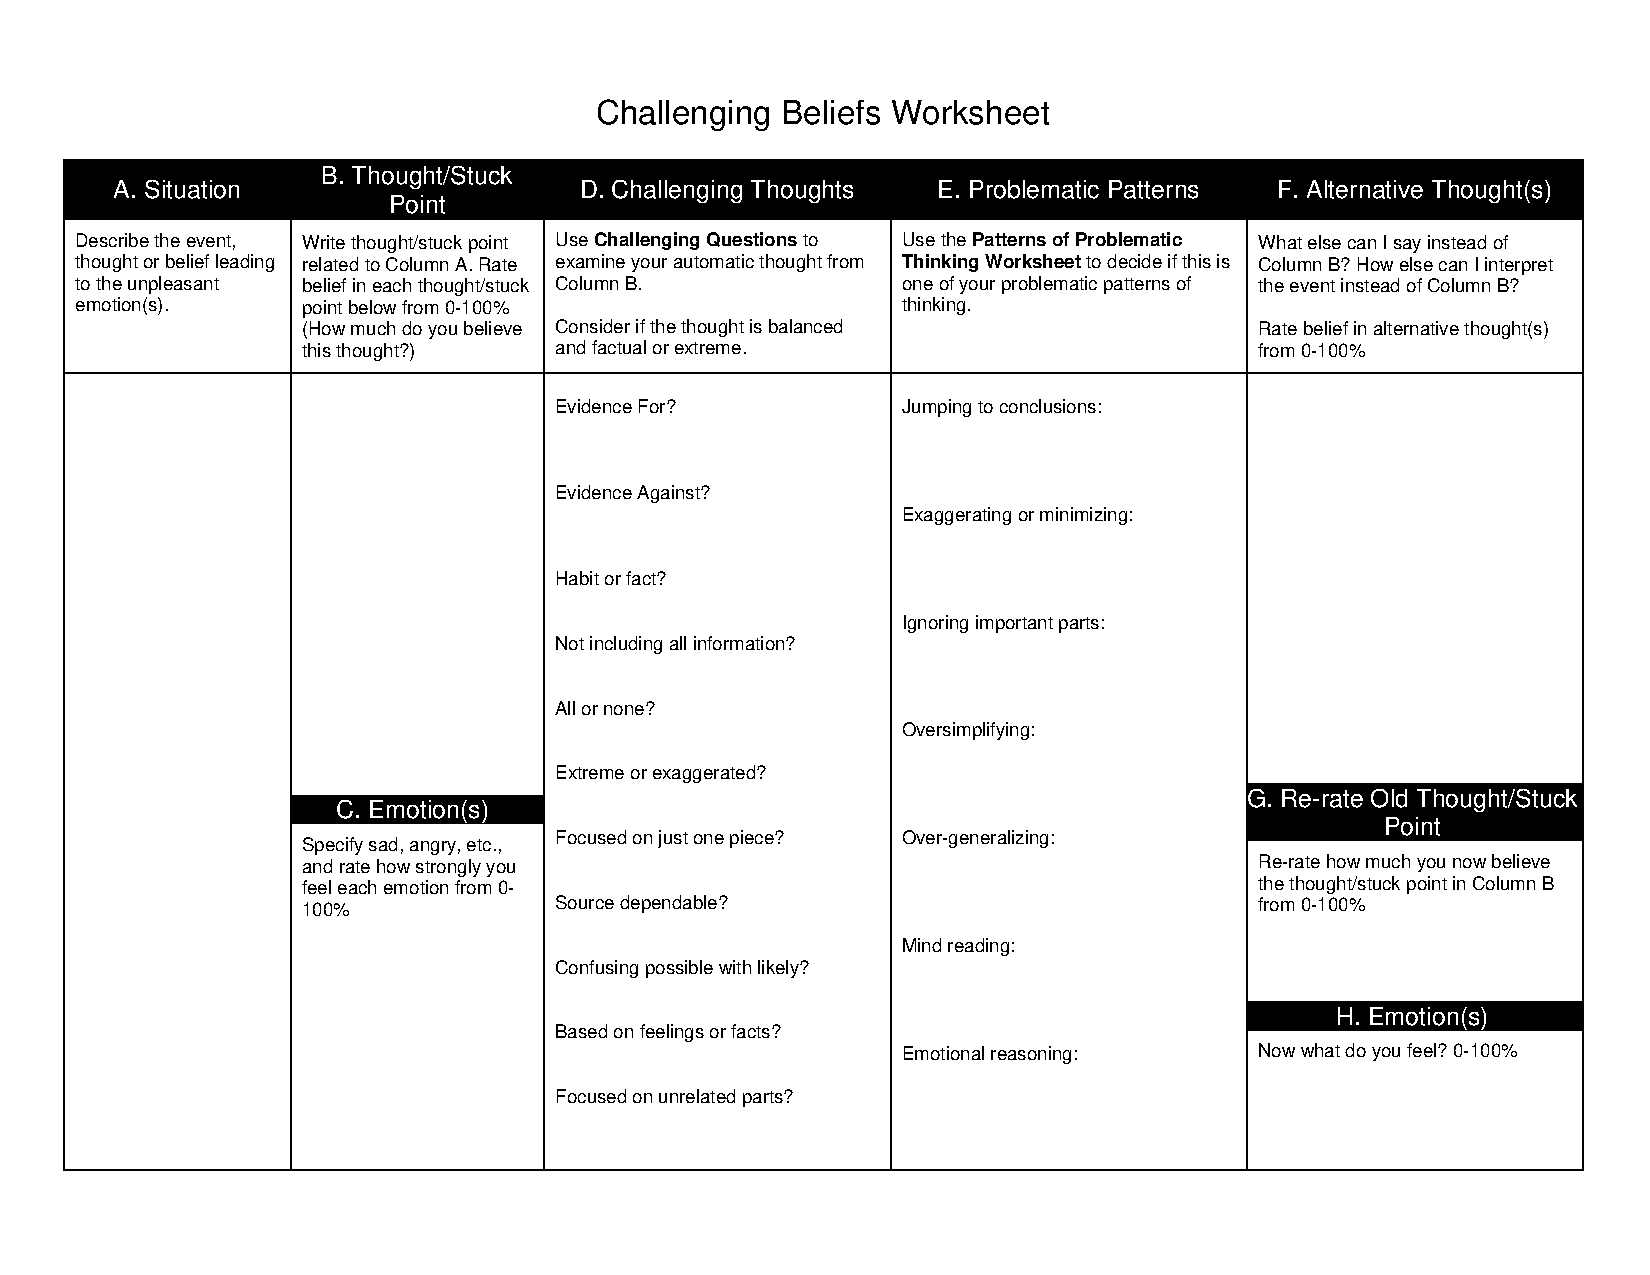
\includepdf[angle={270}]{challenging_beliefs.pdf}
\printbibliography
\addcontentsline{toc}{section}{\bibname}

\end{document}